\documentclass[preprint, 3p,
authoryear]{elsarticle} %review=doublespace preprint=single 5p=2 column
%%% Begin My package additions %%%%%%%%%%%%%%%%%%%

\usepackage[hyphens]{url}

  \journal{Journal of Transport Geography} % Sets Journal name

\usepackage{graphicx}
%%%%%%%%%%%%%%%% end my additions to header

\usepackage[T1]{fontenc}
\usepackage{lmodern}
\usepackage{amssymb,amsmath}
% TODO: Currently lineno needs to be loaded after amsmath because of conflict
% https://github.com/latex-lineno/lineno/issues/5
\usepackage{lineno} % add
\usepackage{ifxetex,ifluatex}
\usepackage{fixltx2e} % provides \textsubscript
% use upquote if available, for straight quotes in verbatim environments
\IfFileExists{upquote.sty}{\usepackage{upquote}}{}
\ifnum 0\ifxetex 1\fi\ifluatex 1\fi=0 % if pdftex
  \usepackage[utf8]{inputenc}
\else % if luatex or xelatex
  \usepackage{fontspec}
  \ifxetex
    \usepackage{xltxtra,xunicode}
  \fi
  \defaultfontfeatures{Mapping=tex-text,Scale=MatchLowercase}
  \newcommand{\euro}{€}
\fi
% use microtype if available
\IfFileExists{microtype.sty}{\usepackage{microtype}}{}
\usepackage[]{natbib}
\bibliographystyle{elsarticle-harv}

\ifxetex
  \usepackage[setpagesize=false, % page size defined by xetex
              unicode=false, % unicode breaks when used with xetex
              xetex]{hyperref}
\else
  \usepackage[unicode=true]{hyperref}
\fi
\hypersetup{breaklinks=true,
            bookmarks=true,
            pdfauthor={},
            pdftitle={A historical analysis of the evolution of active travel behaviour in Canada},
            colorlinks=false,
            urlcolor=blue,
            linkcolor=magenta,
            pdfborder={0 0 0}}

\setcounter{secnumdepth}{5}
% Pandoc toggle for numbering sections (defaults to be off)


% tightlist command for lists without linebreak
\providecommand{\tightlist}{%
  \setlength{\itemsep}{0pt}\setlength{\parskip}{0pt}}




\usepackage{pdflscape}
\usepackage{booktabs}
\usepackage{longtable}
\usepackage{array}
\usepackage{multirow}
\usepackage{wrapfig}
\usepackage{float}
\usepackage{colortbl}
\usepackage{pdflscape}
\usepackage{tabu}
\usepackage{threeparttable}
\usepackage{threeparttablex}
\usepackage[normalem]{ulem}
\usepackage{makecell}
\usepackage{xcolor}



\begin{document}


\begin{frontmatter}

  \title{A historical analysis of the evolution of active travel
behaviour in Canada}
    \author[Some Institute of Technology]{Alice Anonymous%
  \corref{cor1}%
  }
   \ead{alice@example.com} 
    \author[Some Institute of Technology]{Bob Security%
  %
  }
   \ead{bob@example.com} 
    \author[Some Institute of Technology]{Cat Memes%
  %
  }
   \ead{cat@example.com} 
      \affiliation[Some Institute of Technology]{
    organization={Big Wig University},addressline={1 main
street},city={Gotham},postcode={123456},state={State},country={United
States},}
    \cortext[cor1]{Corresponding author}
  
  \begin{abstract}
  Active transportation (AT), defined as self-powered modes such as
  walking and cycling, can help individuals meet the Canadian Society
  for Exercise Physiology's recommendation of 150 minutes of
  moderate-to-vigorous physical activity per week. Despite the potential
  of Canada's Time Use Survey (TUS) from the General Social Survey (GSS)
  to inform AT research, no comprehensive historical analysis of AT
  using all TUS cycles has yet been conducted. This study addresses that
  gap with two objectives: to examine temporal trends in AT by
  destination, travel time, and demographic profiles; and to calibrate
  impedance functions for AT modes across survey cycles and
  destinations. After analyzing and processing over 13,500 AT records
  representing 28 million weighted episodes, we performed descriptive
  analyses and modeled a wide range of impedance functions. Results show
  that ``Home,'' ``Work or study,'' and ``Grocery store'' were the most
  frequent destinations. Walking dominated AT (over 90\% of episodes),
  with median durations rising from 10 to 15 minutes in 2022; for
  cycling, durations rose from 15 to 30 minutes. Since 2010, the share
  of individuals with AT episodes declined, especially among Women+,
  reversing a previous gender pattern. The group cohort between 15 to 24
  years remained as the most active, while adults older than 75 years
  showed steady increases. All fitted impedance functions deviated from
  exponential form, indicating that standard assumptions about patterns
  of distance decay functions may misrepresent AT behavior, particularly
  for short trips. These findings improve our understanding of active
  travel trends and provide empirical support for AT accessibility
  measures and transportation policy.
  \end{abstract}
    \begin{keyword}
    Active mobility \sep Walking \sep Cycling \sep Impedance
function \sep 
    Temporal evolution
  \end{keyword}
  
 \end{frontmatter}

\section{Introduction}\label{introduction}

The Canadian Society for Exercise Physiology (CSEP) recommends that
adults aged 18 to 64 accumulate at least 150 minutes of moderate-to
vigorous-intensity aerobic physical activity per week, in bouts of 10
minutes or more \citep{csep2012}. Moderate-intensity activities are
those that typically cause adults to sweat slightly and breathe harder,
such as brisk walking and bicycling. In contrast, vigorous-intensity
activities cause individuals to sweat more heavily and become out of
breath, including activities like running, basketball, soccer, and
cross-country skiing.

The health benefits of achieving the recommended 150 minutes per week
(approximately 21 minutes per day) include a reduced risk of premature
death \citep{hakim1998effects}, heart disease
\citep{lacroix1996, hakim1999}, stroke \citep{hu2000}, high blood
pressure \citep{dunn1999}, certain cancers, type 2 diabetes
\citep{hu1999}, osteoporosis, overweight, and obesity
\citep{fogelholm2000}. Regular physical activity also contributes to
improved fitness, strength, and mental health, including better morale
and self-esteem \citep{csep2012}.

Active transportation (AT) is an important source of moderate-to
vigorous-intensity physical activity and can help individuals meet
recommended activity levels \citep{bryan2009}. AT refers to
non-motorized and self-powered forms of travel, including walking,
cycling, and the use of aids such as wheelchairs, scooters, e-bikes,
rollerblades, snowshoes, and cross-country skis \citep{csep2012}.
Walking, in particular, is of interest for promoting physical activity
among inactive populations because it is low-cost, easily integrated
into daily routines, requires no special equipment or training, and
carries a relatively low risk of injury compared to more intense
physical activities \citep{hootman2001, bryan2009}. In turn, cycling
provides greater health benefits compared to walking, due to the greater
intensity and duration associated with this mode
\citep{martin2014, barajas2021, borhani2024, celismorales2017}.

Both AT modes, walking and cycling, play a important role in enhancing
and promoting urban sustainability
\citep{hino2014built, lamiquiz2015effects}, making them central to urban
mobility research and policy-making
\citep{vandenbulcke2009mapping, wu2019measuring}. Walking and cycling
accessibility, the ease of reaching destinations and opportunities
\citep{hansen1959, paez2012} by walking and cycling, are closely related
and together contribute to the concept of ``active accessibility'' or
``non-motorized accessibility.'' When incorporated into urban and
transportation planning, they help reduce dependence on private vehicles
and promote healthier, more sustainable travel behavior among residents.

In 2021, Canada released the ``National Active Transportation Strategy''
\citep{canada2021} to support the expansion and enhancement of active
transportation infrastructure in Canada. The federal government
committed \$400 million over five years to build and improve networks of
pathways, bike lanes, trails, and pedestrian bridges. Beyond its
well-established health benefits, the strategy outlines several
additional advantages of expanding AT, including: economic benefits,
such as savings on household transportation costs (e.g., fewer
vehicle-related expenses, trips, and parking needs), increased tourism
and the growth of outdoor and eco-tourism, and increased foot traffic
and spending at businesses accessible via AT; environmental benefits,
such as improved air quality and environmental resilience due to a
higher modal share of AT, reduced land consumption for roads and
parking, and decreased water pollution from runoff due to paved
surfaces; in addition to social benefits, such as increased public space
for social interaction, and improved access to amenities, health care,
education, and social services.

In Canada, the Time Use Survey (TUS) cycles of the General Social Survey
(GSS), administered by Statistics Canada, offer valuable data for
analyzing Canadians' travel behavior \citep{statisticscanada2022}. This
diary-based survey records individuals' activities over 24 hours to
capture societal changes related to living conditions and well-being.
TUS cycles have been conducted every five to seven years since 1986.
Respondents report their main and simultaneous activities, their
duration, location, if other persons accompany them, and, more recently,
whether information technology was used during the activity.

The TUS allows researchers to identify the origin and destination of
trips, travel times, and transportation modes used, providing a valuable
dataset for analyzing active travel behavior. It also offers the
empirical foundation for tools used in transportation analysis, such as
the development of impedance functions for accessibility analysis.

Despite this potential, to our knowledge, no prior studies have
conducted a historical analysis of active travel behavior in Canada
using the full set of TUS GSS cycles. Additionally, the lack of
calibrated impedance functions, especially for destinations beyond work,
poses a challenge for incorporating accessibility into urban and
transportation planning \citep{pereira2023}. The impedance functions
have different forms and all of them serve as a tool to understand the
travel behaviour, since they work as measure of the willingness to
travel a certain distance to achieve a desired destination, where a
service or an opportunity is located
\citep{papa2012gravity, yang2012walking, millward2013active, vale2017influence}.
In this concept, areas with higher accessibility are those characterized
by a lower impedance when traveling to desirable destinations. In
relation to active accessibility, increasing the distance between two
points generally implies in a probability decrease of that trip being
done by walking or biking
\citep{hansen1959, geurs2001accessibility, geurs2004, levinson2005access, cascetta2013new}.
However, more information about the willingness of some individuals to
walk or cycle greater distance is needed, as well as more data on how
distance affects the type and feasibility of the activity, destinations
desirability, and the characteristics of those embarking on the trip in
different situations. Therefore, investigate the evolution and dynamics
of impedance function over time becomes important, since they are easily
impacted by changes in the transportation network or in urban spatial
configurations \citep{iacono2008access, iacono2010}, but also by the
transport behaviour of the population.

Given this context, the present study has two main objectives: to
investigate the Canadian TUS GSS cycles from 1992 to 2022, offering an
overview of AT in terms of primary origins, destinations, travel times,
and the demographic profile of individuals engaging in active travel;
and to calibrate appropriate impedance functions for AT modes (walking
and cycling), considering a wide range of destinations and time periods
in Canadian metropolitan areas. To achieve both objectives, we utilize
data provided by the \texttt{ActiveCA} R package \citep{dossantos2025},
an open data product in the form of an R data package with information
about active travel in Canada. This data product is based on Public Use
Microdata Files of TUS GSS cycles. To build this package, the authors
extracted all walking and cycling episodes and their corresponding
episode weights for GSS cycles, Cycles 2 (1986), Cycles 7 (1992), 12
(1998), 19 (2005), 24 (2010), 29 (2015), and 34 (2022), spanning a
period of almost fourty years. Origins and destinations were labelled,
enabling the investigation of active travel for broad destination
categories and purposes.

We recognize that non-work travel encompasses a range of trip purposes
and diverse traveler behaviors, which makes impedance functions
essential analytical tools for studying non-work accessibility. Grengs
\citeyearpar{grengs2015nonwork} emphasizes the importance of elaborating
distinct functions for each travel purpose, a principle that guides this
analysis. Our investigation covers a variety of trip purposes, ranging
from commutes to homes, workplaces, or educational institutions to
social visits, outdoor activities, business trips, shopping, cultural
outings to libraries, museums, or theaters, dining out, and engaging in
religious practices.

Our research advances the current understanding of active travel
behavior by analyzing of the evolution of travel times and frequency for
AT modes, trends in the prevalence of AT in the Canadian population, and
the development of calibrated impedance functions adapted to different
destinations, periods and AT modes. We ensured the transparency and
reproducibility of our study by sourcing all data from publicly
available repositories. To facilitate collaboration and further
analysis, we developed this paper using literate programming, with the
data analysis code accessible through our GitHub page \emph{(link to be
provided after review)}, in alignment with best practices in spatial
data science \citep{arribas-bel2021}. These contributions enhance the
understanding of active transportation, emphasize its role in shaping
more sustainable mobility strategies, and provide a foundation for
further research and policymaking.

\section{Theoretical background}\label{theoretical-background}

\subsection{Evolution of activity transportation in
Canada}\label{evolution-of-activity-transportation-in-canada}

When analyzing patterns and trends in walking and cycling behavior among
Canadian adults on a national scale, two important studies are
particularly prominent. The first, conducted by Bryan et al.
\citeyearpar{bryan2009}, examined walking behaviours among Canadian
adults aged 18 to 55 using nationally representative cross-sectional
data from the National Population Health Survey and the Canadian
Community Health Survey spanning from 1994/95 to 2007. The authors
calculated the weighted and age-standardized prevalence of walking for
exercise, walking duration, regular walking (defined as walking at least
four times per week), and whether 100\% of leisure-time physical
activity energy expenditure (LTPAEE) was derived from walking. Overall,
70\% of Canadian adults reported walking for exercise at least once
during the previous three months; however, only 30\% reported walking
regularly - a figure that remained relatively stable since 2001. Regular
walking was more commonly reported among women, older adults,
individuals with lower body mass index (BMI), and those in lower-income
households. Similarly, women, older adults, and lower-income Canadians
were more likely to derive 100\% of their total LTPAEE from walking
compared to men, younger adults, and those in higher-income groups. The
study concluded that while walking is a widely practiced form of
physical activity across demographic groups, the prevalence of regular
walking varies considerably by age, sex, BMI, and income.

The second and more recent study, conducted by Borhani et al.
\citeyearpar{borhani2024}, explored active transportation (AT) patterns
in Canada using data from four national health surveys: the National
Population Health Survey (1994--1998), the Canadian Community Health
Survey (2000--2020), the Canadian Health Measures Survey (2007--2019),
and the Health Behaviour in School-aged Children Study (2010--2018).
Their analysis assessed the prevalence of AT participation and time
spent on active trips, focusing on walking and cycling, with results
stratified by age group and sex. The authors noted that inconsistencies
in AT survey questions over time and across surveys posed challenges to
interpreting long-term trends. Even so, they found that females
consistently reported higher levels of walking, while males were more
likely to cycle. Regardless of mode, males reported spending more total
time in AT. Participation in AT decreased with age, with the highest
prevalence observed among youth and the longest durations among young
adults.

\subsection{The Time Use Surveys in
Canada}\label{the-time-use-surveys-in-canada}

TUS surveys provide a valuable source of information on the daily
activities of individuals and households. According to Harms et al.
\citeyearpar{harms2018}, more than 65 countries around the world
(including in Europe, the Americas, Asia, Africa, Australia, and New
Zealand) have conducted together over one hundred TUS. In Canada, the
TUS cycles of the GSS have provided a comprehensive cross-sectional
snapshot of the Canadian population since 1986
\citep{statisticscanada2022}.

Until 2022, Statistics Canada used a telephone-based sampling frame,
which was replaced by a dwelling-based frame in the most recent cycle.
Most respondents to the 2022 TUS answered the survey online. According
to Statistics Canada \citeyearpar{statisticscanada2022}, this new
approach reflected the need to adapt to changes in the use of technology
and the increasing time demands of Canadians, offering respondents
greater flexibility and convenience in completing the survey. However,
it is important to note that significant changes in survey methodology
can affect the comparability of data over time. It is not possible to
determine with certainty whether, or to what extent, the differences
observed in the variables are attributable to actual changes in the
population or to methodological changes in data collection. At all
stages of processing, verification and dissemination, considerable
efforts have been made to produce data with a high level of accuracy and
to ensure that the published estimates meet Statistics Canada's quality
standards. Even so, there is reason to believe that the use of an
electronic questionnaire may have influenced the estimates. The
potential impact of the collection mode was analyzed by Statistics
Canada for a selected set of key questions. Due to the limitations of
the sample size, it was not possible to carry out this analysis for all
the variables. It is worth mentioning that none of the variables used in
this research are listed in Statistics Canada's 2022 Public Use
Microdata File User Guide \citep{statisticscanada2022} as unsuitable for
trend analysis due to differences in data collection mode.

Eligibility for participation requires individuals to be 15 years of age
or older. Each survey cycle spans a full 12-month period, typically from
July to July of the following year. The target population includes all
Canadians aged 15 and older, with the exception of residents of the
Yukon, Northwest Territories, and Nunavut, full-time residents of
institutions, and individuals living on Indigenous reserves. The TUS
covers both rural and urban areas, encompassing metropolitan and
non-metropolitan regions, thereby ensuring a diverse and representative
sample of the Canadian population. For sampling purposes, the ten
provinces of Canada were divided into distinct geographic strata.
Several Census Metropolitan Areas (CMAs) - including St.~John's,
Halifax, Saint John, Montreal, Quebec City, Toronto, Ottawa, Hamilton,
Winnipeg, Regina, Saskatoon, Calgary, Edmonton, and Vancouver - and some
Census Agglomerations (CAs) were treated as separate strata. Additional
strata were created by grouping other CMAs within Quebec, Ontario, and
British Columbia, as well as by categorizing non-CMA areas within each
province into their own distinct strata.

\subsection{Impedance functions in accessibility
measures}\label{impedance-functions-in-accessibility-measures}

Accessibility is the main benefit provided by the transportation system
\citep{pereira2017}, being understood as the potential to access
spatially distributed opportunities \citep{hansen1959, paez2012}. When
computing accessibility measure, is necessary take into account the
challenges associated with this access to different locations and
opportunities. Usually, the effect of travel costs is expressed by
``impedance functions'', also called ``distance decay functions''
\citep{soukhov2024}. Overall, impedance functions are derived from
estimates based on distributions of sample data that reflect variations
in the willingness of individuals to travel different distances to reach
opportunities \citep{li2020approach}. Their objective is to describe the
decrease in the intensity of interaction as the cost of travel between
locations increases. The cost of travel is usually measured in terms of
the distance between the places of origin and destination, or in terms
of the time spent reaching the destination from the point of origin.

Examining the impedance functions across different modes of transport
and destinations is a good way to understand the travel behavior
associated with each mode, while also helping to examine allegations
about travel behavior. Current interest in creating ``livable''
communities often relies on broad assumptions about individuals'
willingness to walk or bike to different destinations. For example, it
is commonly assumed that people are generally willing to walk up to a
quarter mile to access most places \citep{untermann1984, larsen2010}.
Similarly, the recent ``15-minute city'' concept proposes that the
majority of daily necessities should be accessible by walking or cycling
within 15 minutes \citep{moreno2021}.

Different categories of accessibility measures have been developed, such
as indicators based on actives, infrastructure, individuals and
utilities \citep{geurs2004, paez2012}. The family of gravity-based
accessibility have been widely used in active modes \citep{miller2005}.
Many gravity-based accessibility measures derive from the work of Hansen
\citeyearpar{hansen1959}, represented in (Equation
\ref{eq:accessibility-equation}), in which an impedance function weights
opportunities:

\begin{equation}
A_{i} = \sum_{j=1}^J O_j .f(c_{ij})
\label{eq:accessibility-equation}
\end{equation}

The accessibility score \(A_{i}\) at each origin \(i\) is obtained by
summing up the opportunities \(O\) available at destination \(j\), where
\(i\) and \(j\) are sets of spatial units in a region. However, the
number of opportunities in each destination is gradually discounted as
travel costs become higher and the rate at which this weight decreases
is determined by a decay function. \(f(c_{ij})\) represents the
impedance during the trip from origin \(i\) to destination \(j\) and
\(c_{ij}\) reflects the generalized travel cost, potentially
encompassing factors such as time, distance and effort. In this way, the
impedance function \(f(c_{ij})\) allows the accessibility analyst to
define a measure of travel behavior with precision: the relationship
between the ``population'' at an origin and where they normally want to
or can go to reach ``opportunities'' at destinations. The definition of
the impedance function \(f(c_{ij})\) is very important from this
perspective \citep{soukhov2024}.

Since the beginning applications of the gravity-accessibility models, a
range of impedance functions have been applied to describe the
distribution of walking and cycling trips, whether for general or
specific purposes
\citep{iacono2008access, iacono2010, larsen2010, yang2012walking, millward2013active, vale2017influence, li2020approach}.
Selecting an appropriate impedance function can be challenging and
results in a diverse range of cost decay functions that are employed as
impedance functions in accessibility measures, including threshold
functions and smooth cost decay functions (e.g., log-normal, normal,
gamma, and exponential function)
\citep{de2009exponential, reggiani2011accessibility, osth2016new}.

Another type of family of accessibility measures are \emph{cumulative
opportunity} metrics, commonly referred to as isochronous indices. The
binary function Equation \ref{eq:cumulative-equation} forms the basis of
the cumulative opportunities measure approach. This function determine
accessibility by summing up the number of opportunities available within
a specific threshold of travel time or distance from a reference point,
without discounting the potential of the trip in relation to the
associated cost. They use a rectangular function, categorizing the trip
as ``acceptable'' within certain limits and ``unacceptable'' beyond
them. One of the main complexities of these metrics is deciding what the
appropriate threshold point is. This decision may be based on the
prevailing mobility patterns of the population or may reflect
established norms, conventions or informed projections of the
researcher. Note that the cumulative opportunity measure can be
understood as a special case of a gravity-based measure in which the
weight of each opportunity is defined by a binary function, rather than
a gradually decaying function \citep{pereira2023}.

\begin{equation}
C_{ij} =
\begin{cases}
  1 & \text{if } c_{ij} \le x \\
  0 & otherwise
\end{cases}
\label{eq:cumulative-equation}
\end{equation}

Among the various mathematical forms that can represent impedance
functions, the negative exponential function is the dominant choice in
accessibility research
\citep{hansen1959, apparicio2008comparing, iacono2008access, larsen2010, millward2013active}.
Its high adoption can be attributed mainly to its ability to give
greater weight to nearby opportunities, and greater weight to distant
opportunities - a highly relevant characteristic for active modes of
transportation, such as walking and cycling. When Hansen
\citeyearpar{hansen1959} introduced their accessibility measure, the
author applied and indicated the use of exponential distributions
\((e ^ {-\beta x})\) as the impedance function. After this, several
other studies
\citep{fotheringham1989spatial, de2009exponential, iacono2010, signorino2011gravity, prins2014many}
use the negative exponential function after comparison with empirical
trip distribution data.

Researchers can adopt other forms of impedance functions when
calculating the distance decay effect in accessibility analysis. One of
these options is to adopt a probability density function (PDF)
\citep{soukhov2024}. Using a PDF, \(f()\) can be interpreted as the
probability density of a trip occurring for each value of travel cost
\(c_{ij}\). If a graph of the PDF (y-axis) is plotted against the travel
cost \(c_{ij}\) (x-axis), the probability of a trip occurring between a
given range of \(c_{ij}\) is the area under the curve. In this case, the
total area under the PDF curve always sums to 1, meaning that there is
100\% probability that the trip will occur between the minimum and
maximum \(c_{ij}\).

Dunn et al. \citeyearpar{dunn2023} presented a set of distributions that
serve as PDFs. From their survey, we selected some options for \(f()\)
commonly used in accessibility research and their impact on the number
of opportunities (the sum of opportunities) at specific travel costs
\(c_{ij}\), namely: uniform, negative exponential, gamma, normal, and
lognormal distributions.

\begin{itemize}
\tightlist
\item
  \textbf{Uniform distribution}: The uniform distribution or rectangular
  PDF looks very similar to the binary function, since it only returns
  one of two values, but ensure that area under the curve for the range
  of \(c_{ij}\) is 1. The uniform distribution PDF is shown in (Equation
  \ref{eq:uniform-equation}). The parameters to be calculated are
  \(c_{max}\) and \(c_{min}\), which represent the maximum and minimum
  travel costs that describe the observed or assumed willingness to
  reach destinations. In this distribution, all values within the
  interval are equally likely, and all values outside the interval have
  probability 0, assuming that the population's potential to interact
  with these opportunities is zero. Usually, \(c_{min}\) has value 0.
\end{itemize}

\begin{equation}
f(c_{ij})^{uniform} =
\begin{cases}
  \frac{1}{c_{max} - c_{min}} & \text{for } c_{min} \le c_{ij} \le c_{max} \\
  0 & \text{otherwise}
\end{cases}
\label{eq:uniform-equation}
\end{equation}

\begin{itemize}
\tightlist
\item
  \textbf{Exponential distribution}: The exponential distribution PDF
  equation is given by Equation \ref{eq:exponential-equation}. This
  model suggests that impedance decreases exponentially with increasing
  cost \((c_{ij})\). The parameter \(\beta\) represents the decay rate,
  with higher values indicating a faster decrease in accessibility with
  increasing cost. As already mentioned, this function is widely used
  due to its simplicity and ability to model the rapid drop-off in
  accessibility over distance.
\end{itemize}

\begin{equation}
f(c_{ij}) = e^{-\beta c_{ij}} \text{ with } c_{ij} \ge 0
\label{eq:exponential-equation}
\end{equation}

\begin{itemize}
\tightlist
\item
  \textbf{Gamma distribution}: The gamma distribution PDF equation is
  presented by the Equation \ref{eq:gamma-equation}. Where
  \(\Gamma(\alpha)\) is the gamma function to be estimated. In this
  case, the probability is typically low at low cost, higher at medium
  cost, and low again at high cost. The higher the \(\sigma\) (scale
  rate) parameter, the higher the probability that the majority of trips
  will be in the low cost range. So at low values of the \(\sigma\)
  (scale rate) parameter, the same probability is spread over a wider
  range of travel costs. For the \(\alpha\) (shape) parameter, the
  higher the value, the higher the probability density of trips with a
  higher average cost \citep{soukhov2024}.
\end{itemize}

\begin{equation}
f(c_{ij}) = 
   \begin{cases}
\frac{1}{\sigma^\alpha\Gamma(\alpha)} c_{ij}^{\alpha-1} e^{\frac{-c_{ij}}{\sigma}} & \text{if } 0 \leq c_{ij} <      \infty  \text{ and } \alpha, \sigma > 0 \\ 0 & \text{otherwise}
   \end{cases}
\label{eq:gamma-equation}
\end{equation}

\begin{itemize}
\tightlist
\item
  \textbf{Lognormal distribution}: The normal distribution, also often
  called the Gaussian distribution, is suitable when the travel cost is
  found to be distributed normally. The normal distribution has the PDF
  form displayed in Equation \ref{eq:normal-equation}. In this equation,
  \(\mu\) and \(\sigma\) are the mean and standard deviation of the
  distribution and need to be estimated together to control the shape of
  the normal curve. In this distribution, about 68\% of the observations
  will fall within 1 standard deviation of the mean, about 95\% will
  fall within 2 standard deviations, and about 99.7\% will fall within 3
  standard deviations of the mean. In this case, the values close to the
  mean will have the highest probability.
\end{itemize}

\begin{equation}
f(c_{ij}) = \frac{1}{\sqrt{2\pi} \sigma c_{ij}} e^{-\frac{(\ln c_{ij} - \mu)^2}{2\sigma^2}}
\label{eq:normal-equation}
\end{equation}

\begin{itemize}
\tightlist
\item
  \textbf{Lognormal distribution}: In many cases, the logarithm of the
  travel cost is found to be distributed normally. The lognormal
  distribution has the PDF form displayed in Equation
  \ref{eq:lognormal-equation}. It this equation, \(\mu\) and \(\sigma\)
  are the mean and standard deviation of the logarithm, and need to be
  estimated for together control the shape of the log-normal curve.
  Similar to the gamma function, the probability is typically low at low
  cost, higher at medium cost, and low again at high cost.
\end{itemize}

\begin{equation}
f(c_{ij}) = \frac{1}{\sqrt{2\pi} \sigma c_{ij}} e^{-\frac{(\ln c_{ij} - \mu)^2}{2\sigma^2}}
\label{eq:lognormal-equation}
\end{equation}

As the complexity of the PDF increases, so does the flexibility to
explain travel behaviour. However, the estimation of the impedance
function parameters needs to be calibrated if the accessibility
estimates are to be representative of people's travel behaviour. This
requires additional travel behaviour data to be used in the calibration
process.

\section{Materials and Methods}\label{materials-and-methods}

To investigate the historical active travel behavior in Canada, we
analyzed six GSS Time Use cycles: Cycles 7 (1992), 12 (1998), 19 (2005),
24 (2010), 29 (2015) and 37 (2022). We excluded Cycle 2 (1986) from our
analysis because this survey did not specify whether the respondent
lived in a metropolitan area and did not present cycling as a option of
transportation mode, although this cycle is notable for having been the
first national random sample to examine Canadian time-use patterns. This
paper is a direct application of the ready-to-use data set provided by
the \texttt{ActiveCA} data package \citep{dossantos2025}, which is based
on the Main and Episode files from the GSS Public Use Microdata Files.
The Main file contains questionnaire responses and associated data from
participants, while the Episode files provided detailed information
about every activity episode reported by the respondents.

The methodology involves two main steps. The first step employs
descriptive analysis of AT episodes to identify typical travel times
across destinations and years, comparing their temporal evolution and
identifying differences in AT episodes through statistical tests, and
assess the active population in terms of sex and age group. The second
step calculates and analyzes impedance functions for each combination of
cycle, destination, and AT mode.

To facilitate collaboration and further analysis, we updated the
\texttt{ActiveCA} R Package to include the methodology to obtain
impedance functions from the raw data files (GSS surveys). Additionally,
we created this paper using literate programming in which the R markdown
code to fully reproduce this article is available on our GitHub
repository \emph{(include after the review)}, in line with the best
practices of spatial data science \citep{arribas-bel2021, paez2021}.

\subsection{Analyzing active travel
episodes}\label{analyzing-active-travel-episodes}

A TA episode refers to a walking or cycling activity that a person did
the day before the TUS interview. For each selected cycle of the GSS
surveys, we reviewed the episode files to identify cases with activities
listed as walking or cycling, selecting the locations immediately before
and after the mobility episode. With this process, we were able to
identify the origin and the destination of the active travel episode. We
labeled the code variables with their appropriate descriptions,
identifying the transportation mode, activity/reason of the travel, as
well the province and urban classification of the respondent's residency
(if the respondent lives in a CMA or in a Census Agglomerations).

Additionally, it was necessary to guarantee the data consistency across
the surveys, since they have employed a variety of variable coding
schemes. The range of activities and destinations considered in the
surveys changed from 1992 to 2022. In 1992, there were only three
options of origin/destination location available to the respondent:
their home, other's home and work or study. In its turn, the most recent
survey (2022) counts with twelve possible destination, including sport
area (sports centre, field or arena), restaurant (including bar and
club), health clinics (medical, dental or other health clinic), grocery
stores (including other types of stores and malls) and more. In order to
achieve uniformity, the activity categories from 2005, 2010, 2015, and
2022 were synchronised, and a similar process was employed for those
from 1992 and 1998. For the preceding years (1992, and 1998), the trip
origins and destinations were classified as ``Home,'' ``Other's home,''
and ``Work or school.'' In the subsequent years (2005, 2010, 2015, and
2022), these categories were expanded to include ``Business,''
``Restaurant'' ``Place of worship,'' ``Grocery store''
``Neighbourhood,'' ``Outdoors,'' ``Cultural venues'' (such as library,
museum and theatre), and ``Sport area.''

Statistical analysis was used to characterize active travel episodes
using cross-tabulations and graphs. Summary statistics and visualization
techniques, including median values as a measure of typical value and
box plots, were employed to describe active travel across years,
destinations, and transportation modes. To assess the statistical
significance of potential temporal differences in the empirical episode
data set for each destination, we applied the Kruskal-Wallis test - a
test that evaluates differences in the medians of the empirical data.
This test was chosen because it does not assume a normal distribution
for the data, an important consideration since we made no assumptions
about the distribution of the empirical data.

\subsection{Analyzing the population with active travel
records}\label{analyzing-the-population-with-active-travel-records}

After assessing the active travel episodes, we analyzed the population
with records of active travel for each year of the analysis, stratifying
the analysis by gender and age group. To stratify by gender, we adopted
the definition used in the most recent TUS (2022), which was the first
in the series to consider gender - recognizing a broader spectrum of
gender identities - instead of biological sex, which had previously been
limited to female and male categories. In the 2022 survey, due to the
small size of the non-binary population, data aggregation was necessary
to protect the confidentiality of respondents
\citep{statisticscanada2025}. As a result, information from the TUS 2022
is disseminated using a two-category gender variable. In this framework,
individuals identifying as non-binary are distributed across the two
other gender categories and are denoted by the ``+'' symbol. The
category ``Men+'' includes men (and/or boys) as well as some non-binary
persons, and the category women+ includes women (and/or girls) as well
as some non-binary persons.

We recognize that biological sex does not always align with gender
identity. However, to enable comparison across survey years, we assumed
that individuals recorded as ``female'' in earlier surveys correspond to
women+, and those recorded as ``male'' correspond to ``Men+''. We
acknowledge that this approach does not fully capture gender diversity,
particularly for trans and non-binary individuals, due to limitations in
how gender was recorded in earlier surveys.

We also stratified the analysis by age group. To ensure the consistency
across all survey years, we defined the following cohorts: ``15 to 24
years'', ``25 to 34 years'', ``35 to 44 years'', ``45 to 54 years'',
``55 to 64 years'', ``65 to 74 years'', and ``75 years and over''.

After defining the gender and age group categories, we identified the
population with and without at least one active travel episode,
considering both modes (walking and cycling). To complete the population
analysis, we measured and examined the temporal evolution of the number
of active trips per person for each survey year, considering both the
active population and the general population. We also analyzed the
number of walking episodes per person who reported walking activity, and
the number of cycling episodes per cyclist, to identify possible trends
within each AT mode. Finally, we compared the average duration of active
travel episodes to observe changes over time.

\subsection{Estimating impedance function
parameters}\label{estimating-impedance-function-parameters}

We applied the \texttt{fitdistrplus} package
\citep{delignette2015fitdistrplus} to calculate the best PDF for every
destination, mode of transportation and survey year, between the
options: uniform, negative exponential, gamma, normal, and lognormal
distributions. In order to calculate the impedance functions, two
filters were applied in the GSS data set. The first is that we excluded
all trips with travel times higher than 100 minutes (1.5 hours). An
exploratory data analysis showed that, taking into account all the
walking and cycling records (19,166 in total), less than 0.73\% of them
have a trip duration higher than this limit. When considering the
weights of this episodes, travel times higher than 100 minutes
represented 0.93\% of the episodes. Due to the description of the
activities, it was also possible to know that trips with a duration
higher than 100 minutes are mainly composed of hiking and camping
episodes. The second filter was realized to select only the population
living in a larger urban population centre. We decided to apply this
restriction because the travel behaviour of residents of CMA and CA
areas tends to be very different from those outside these large urban
centres in terms of active travel.

\section{Results and discussion}\label{results-and-discussion}

\subsection{Descriptive analysis}\label{descriptive-analysis}

\subsubsection{Active transportation
episodes}\label{active-transportation-episodes}

After applying the filters to the GSS surveys, we obtained a total of
19,166 cases of active travel episodes. However, GSS surveys apply a
probability sampling methodology, in which each episode or person
selected in the sample represents several other episodes or persons not
in the sample. The number of episodes and persons represented by a
episode or person is determined by the weight or weighting factor.
Because of this, every estimates of the number of episodes or persons
need to be calculated applying the corresponding weighting factors.

Considering the weights, the 19,166 episodes represent a total of
28,066,620 episodes. Table \ref{tab:episodes-count-percentages} contains
the weighted number of episodes about walking and cycling trips between
1992 and 2022, obtained from the GSS cycles. The year 2010 is the year
with the most episodes, with 7,116,460 episodes (representing 25.36\% of
the total). The year 1992 has the lowest number of episodes, with only
1,767,041 episodes, representing 6.3\% of the total. The most recent
survey, 2022, counted with 5,335,510 episodes (19.01\% of the total).

When analyzing the two AT modes, walking episodes account for 91.56\%,
while the remaining 8.44\% are cycling episodes. The most recent survey
(2022) showed that cycling trips accounted for almost 10\% of active
travel episodes, reinforcing an increasing trend in the cycling
participation since 2005 - the year that marked the lowest
representation, as opposed to 1992, when bicycle episodes marked the
highest participation in all years (13\%).

\begin{table}
\centering
\caption{\label{tab:bulding table-01}\label{tab:episodes-count-percentages}Weighted number of episodes identified in each active transportation mode by year.}
\centering
\fontsize{10}{12}\selectfont
\begin{tabular}[t]{lrrrrrr}
\toprule
\multicolumn{1}{c}{ } & \multicolumn{2}{c}{Cycling} & \multicolumn{2}{c}{Walking} & \multicolumn{2}{c}{Both modes} \\
\cmidrule(l{3pt}r{3pt}){2-3} \cmidrule(l{3pt}r{3pt}){4-5} \cmidrule(l{3pt}r{3pt}){6-7}
Year &  & (\%) &  & (\%) &  & (\%)\\
\midrule
1992 & 230316.9 & 13.03 & 1536724 & 86.97 & 1767041 & 6.30\\
1998 & 156123.1 & 8.81 & 1616938 & 91.19 & 1773061 & 6.32\\
2005 & 472839.5 & 7.68 & 5679938 & 92.32 & 6152778 & 21.92\\
2010 & 559295.6 & 7.86 & 6557165 & 92.14 & 7116460 & 25.36\\
2015 & 475626.6 & 8.03 & 5446145 & 91.97 & 5921772 & 21.10\\
\addlinespace
2022 & 474128.9 & 8.89 & 4861381 & 91.11 & 5335510 & 19.01\\
Total & 2368330.7 & 8.44 & 25698290 & 91.56 & 28066620 & 100.00\\
\bottomrule
\end{tabular}
\end{table}

Figure \ref{fig:figure-destmodeyearperc} shows the percentage of each
destination by year and by mode of transport. For all the years
analyzed, `Home' is the most common travel destination, regardless of
whether the mode of transport considered is walking or cycling, with
levels above 40\%. After that, `Work or school' appears as the second
most common destination, especially for journeys by bicycle, with a peak
of almost 36\% of trips by bicycle in 1998, followed by a high drop to
23\% in 2005. Along with the two destinations already mentioned,
`Other's home' is the only other destination present in the GSS surveys
since 1992. This last destination seems to be a destination with a
higher share when it comes to walking trips, but for both modes of
transportation it seems that respondents are going less and less to
other people's homes - a fact that can be explained by new communication
technologies, in which a person does not need to visit another person's
home to keep in touch with them.

\begin{figure}
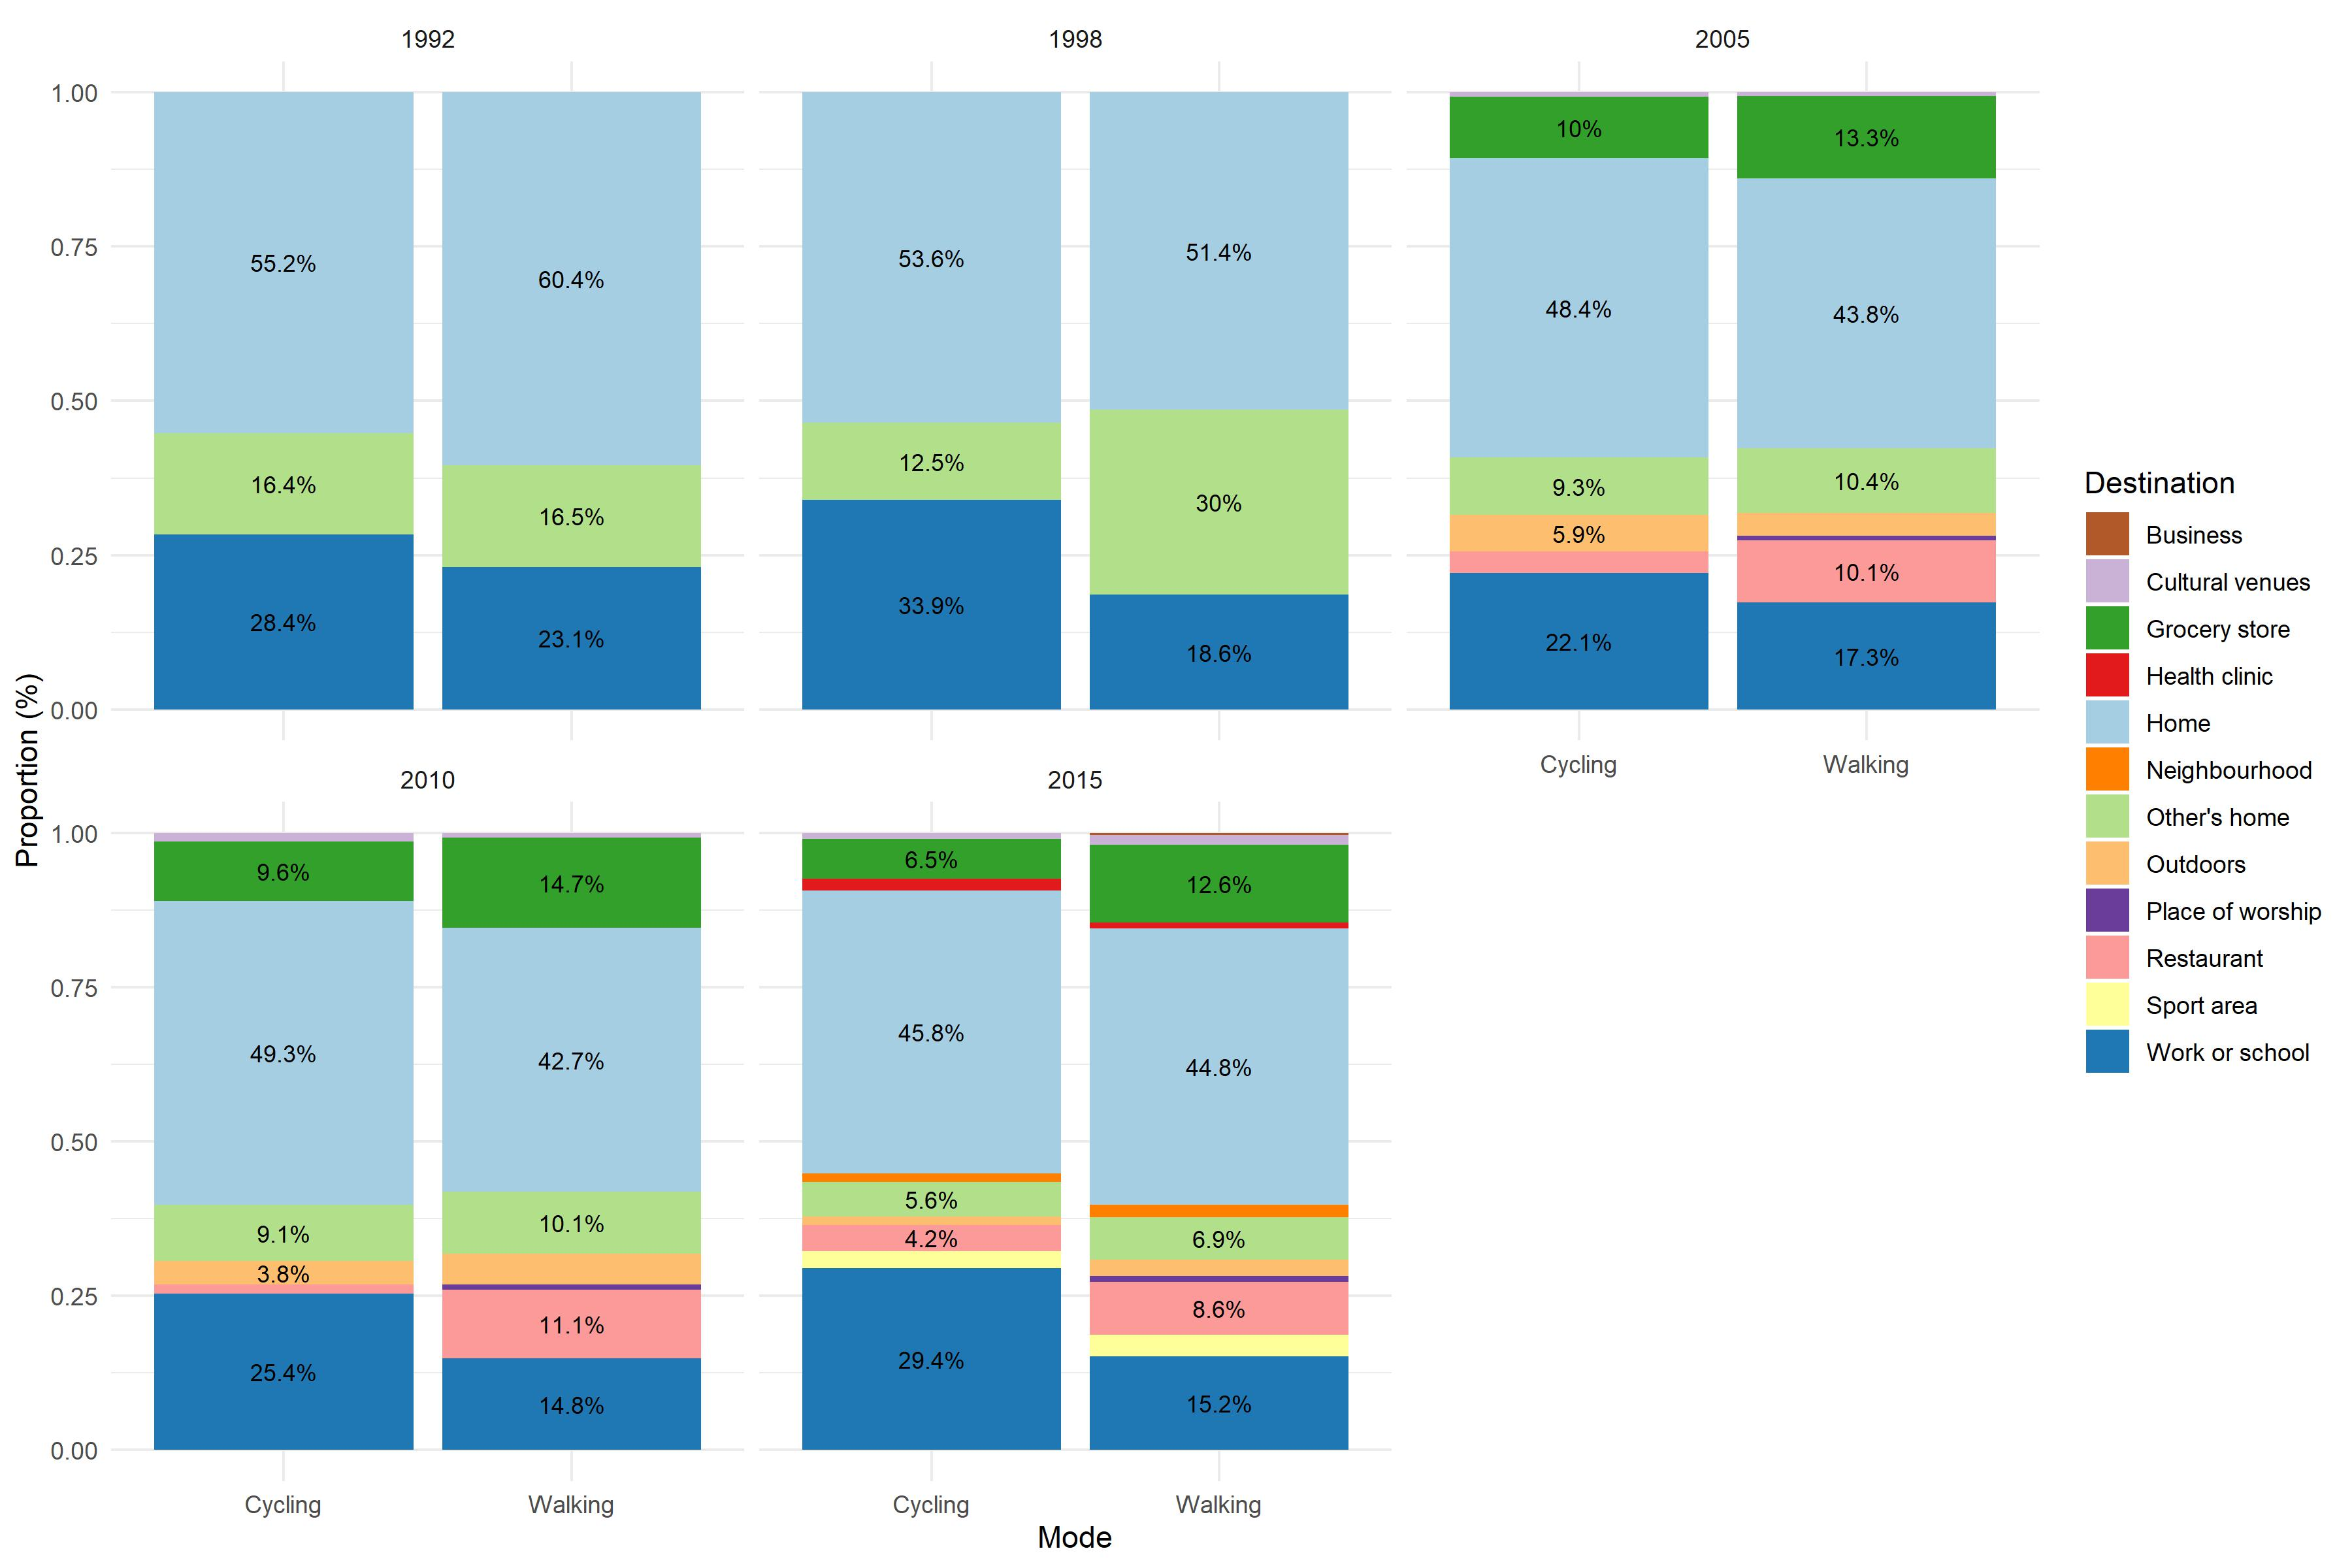
\includegraphics[width=1\linewidth]{figures/destination_percentual} \caption{Percentage of walking and cycling trips categorized by destination and year.}\label{fig:figure-destmodeyearperc}
\end{figure}

After 2005, the expansion of the destination highlights some new popular
locations. For example, `Grocery store' appears as the third most chosen
destination, varying from almost 10\% in 2005 to 14.3\% in 2022 for
cycling trips and from 12\% to 12.6\% for walking trips. When
considering walking trips, `Restaurants' appears as another well chosen
destination and, in the case of cycling trips, `Outdoors' appears as a
well chosen destination.

The maximum time spent on walking trips varied between 90 and 100
minutes across the years (Table \ref{tab:decrip-analysis}) - it is
important to remember that trips with duration greater than 100 minutes
were excluded from the analysis. The mean walking time also varies,
starting at 20 minutes in 1992, dropping to 12 minutes between 1992 to
2005, and increasing survey after survey until it reaches 18 minutes in
2022. However, it is known that the mean is a statistic that is highly
influenced by extreme values. For this reason, we analyze the median
travel time, as it is more representative of the typical travel time.
The median time spent walking was 10 minutes in 1992, dropped to 5
minutes in 1998, remained constant at 10 minutes from 2005 to 2015, and
increased to the highest level in 2022, to 15 minutes.

\begin{table}
\centering
\caption{\label{tab:table-02}\label{tab:decrip-analysis}Descriptive statistics for episodes with active transport records.}
\centering
\fontsize{10}{12}\selectfont
\begin{tabular}[t]{>{}llcccccc}
\toprule
\multicolumn{2}{c}{ } & \multicolumn{6}{c}{Year} \\
\cmidrule(l{3pt}r{3pt}){3-8}
Mode & Statistic & 1992 & 1998 & 2005 & 2010 & 2015 & 2022\\
\midrule
 & Maximum & 90 & 100 & 100 & 90 & 95 & 90\\

 & Mean & 20 & 12 & 12 & 13 & 16 & 18\\

 & Median & 10 & 5 & 10 & 10 & 10 & 15\\

 & Minimum & 5 & 1 & 1 & 1 & 5 & 5\\

\multirow[t]{-5}{*}{\raggedright\arraybackslash \textbf{Walking}} & Standard deviation & 19 & 13 & 12 & 13 & 13 & 15\\
\cmidrule{1-8}
 & Maximum & 90 & 80 & 95 & 100 & 90 & 60\\

 & Mean & 21 & 28 & 20 & 18 & 24 & 30\\

 & Median & 20 & 25 & 15 & 10 & 20 & 30\\

 & Minimum & 5 & 2 & 1 & 2 & 5 & 5\\

\multirow[t]{-5}{*}{\raggedright\arraybackslash \textbf{Cycling}} & Standard deviation & 20 & 19 & 16 & 16 & 15 & 14\\
\bottomrule
\end{tabular}
\end{table}

For cycling trips, the maximum travel time ranges from 60 to 100
minutes. Until 2022, maximum travel times had a similar pattern to
walking trips, but the new survey showed that the maximum travel time
for cycling trips was the lowest when considering all years for both
modes (walking and cycling). The average median travel time fluctuated
between the periods, starting at 20 minutes in 1992 and peaking at 30
minutes in 2022. As was also the case with the walking travel times,
these results show a trend of increasing for cycling trip duration
throughout the years. The analysis of travel time statistics alone does
not fully explain the reasons behind these fluctuations in travel time
over the years. However, it is likely that these variations reflect
changes in bicycle technology or cyclist behavior.

Figure \ref{fig:figure-boxplot} presents box plots showing the
distribution of travel times for active transport modes over the years,
categorized by destination. During the period studied, the typical
duration of walking trips was consistently shorter than that of cycling
trips. While we can compare the temporal evolution of travel times, some
destinations appear only in the two most recent surveys, such as
``Neighborhood,'' ``Health clinic,'' ``Sports area,'' and ``Business.''
The first three showed a constant median walking travel time of 10
minutes in both surveys, while the median travel time to ``Business''
increased from 10 to 15 minutes. For cycling trips, ``Business''
recorded no trips, while ``Neighborhood'' had a typical travel time of
30 minutes in 2015 but no records for 2022. ``Health clinic'' showed a
constant cycling travel time of 15 minutes, and ``Sports area'' doubled
its typical duration, from 15 to 30 minutes.

\begin{figure}

\includegraphics[width=1\linewidth]{figures/destination_boxplots} \caption{Percentage of walking trips categorized by origin and destination}\label{fig:figure-boxplot}
\end{figure}

For the other destinations, starting with walking trips, we note a trend
of increasing travel times for almost all destinations, with an increase
observed at least in the most recent survey (2022). ``Restaurants'' and
``Outdoors'' both increased their typical travel time from 5 minutes in
2005 to 10 minutes in 2022; ``Other's home'' rose to 10 minutes in 2022
after remaining at 5 minutes since 1992; ``Place of worship'' increased
from 10 minutes in 2005 to 20 minutes in 2022; and ``Cultural venues''
rose from 10 minutes in 2005 to 20 minutes in 2022. The three most
popular types of destinations - ``Home,'' ``Work or school,'' and
``Grocery store'' - had an increase to 15 minutes after decades of
stabilization at 10 minutes. In general, while ``Place of worship'' and
``Cultural venues'' displayed the highest median travel times of 20
minutes, the overall median walking time cutoff across all surveys
appears to be 10 minutes, with most trips occurring below this threshold
- except for 2022, when this limit was increased by 15 minutes. No
destination shows a decrease in typical (median) travel time.

For cycling trips, only ``Cultural venues'' did not show an increase in
typical travel time when comparing 2022 to the previous years. In this
case, the travel time dropped from 25 minutes in 2010 to 15 minutes in
2015, although it remained higher than the 2005 value (10 minutes), and
no trips were recorded in the most recent survey (2022). ``Other's
home'' is the other destination with no cycling records for the 2022
survey. An increasing trend in travel times is evident for destinations
such as ``Grocery store'' (rising from a median of 10 to 60 minutes
between 2005 and 2022) and ``Restaurant'' (rising to a median of 30
minutes in 2022).

Other destinations seem to follow a similar pattern of increasing travel
time, where higher values were recorded in earlier survey cycles,
dropped over time, and then rose again in the most recent surveys. This
is the case for ``Home,'' which reached its highest typical travel time
of 25 minutes after dropping to 10 minutes in 2010. It is also worth
mentioning ``Work or school,'' which had a typical cycling travel time
of 15 minutes in 1992, peaked at 30 minutes in 1998, dropped back to 15
minutes in 2005 and 2010, and then increased to 25 minutes in 2022. In
this case, no destination shows a decrease in typical (median) travel
time.

Figures \ref{fig:walking-heatmap} and \ref{fig:cycling-heatmap} show
walking and cycling trips from 1992 to 2022 through heat maps. These
maps use color gradients to represent the percentage of trips between
origins and destinations, with darker colors indicating higher
percentages and lighter colors representing less frequent routes. In
1992, walking trips with `Home' as both the origin and destination made
up the majority, accounting for almost 31\% of all walking trips. These
trips often involved leisure activities, like short walks or dog
walking. Following this, trips from `Home' to `Work or school' comprised
18\% of walking trips. Overall, `Home' is the principal hub, either as
an origin or destination, with only 7\% of trips not involving `Home.'
In 2005, trips with origins or destinations involving `Home' and `Work
or school' remained as the most common, but the introduction of new
destinations led to a more dispersed trip distribution. Together, these
two combinations accounted for 25\% of all trips. In the most recent
survey, the most common trip was from ``Home'' to ``Work or school''
(17\%), followed by the return trip from ``Work or school'' to ``Home''
(13\%). After that, trips between ``Home'' and the ``Grocery store''
accounted for 20\% when both directions are combined.

\begin{figure}
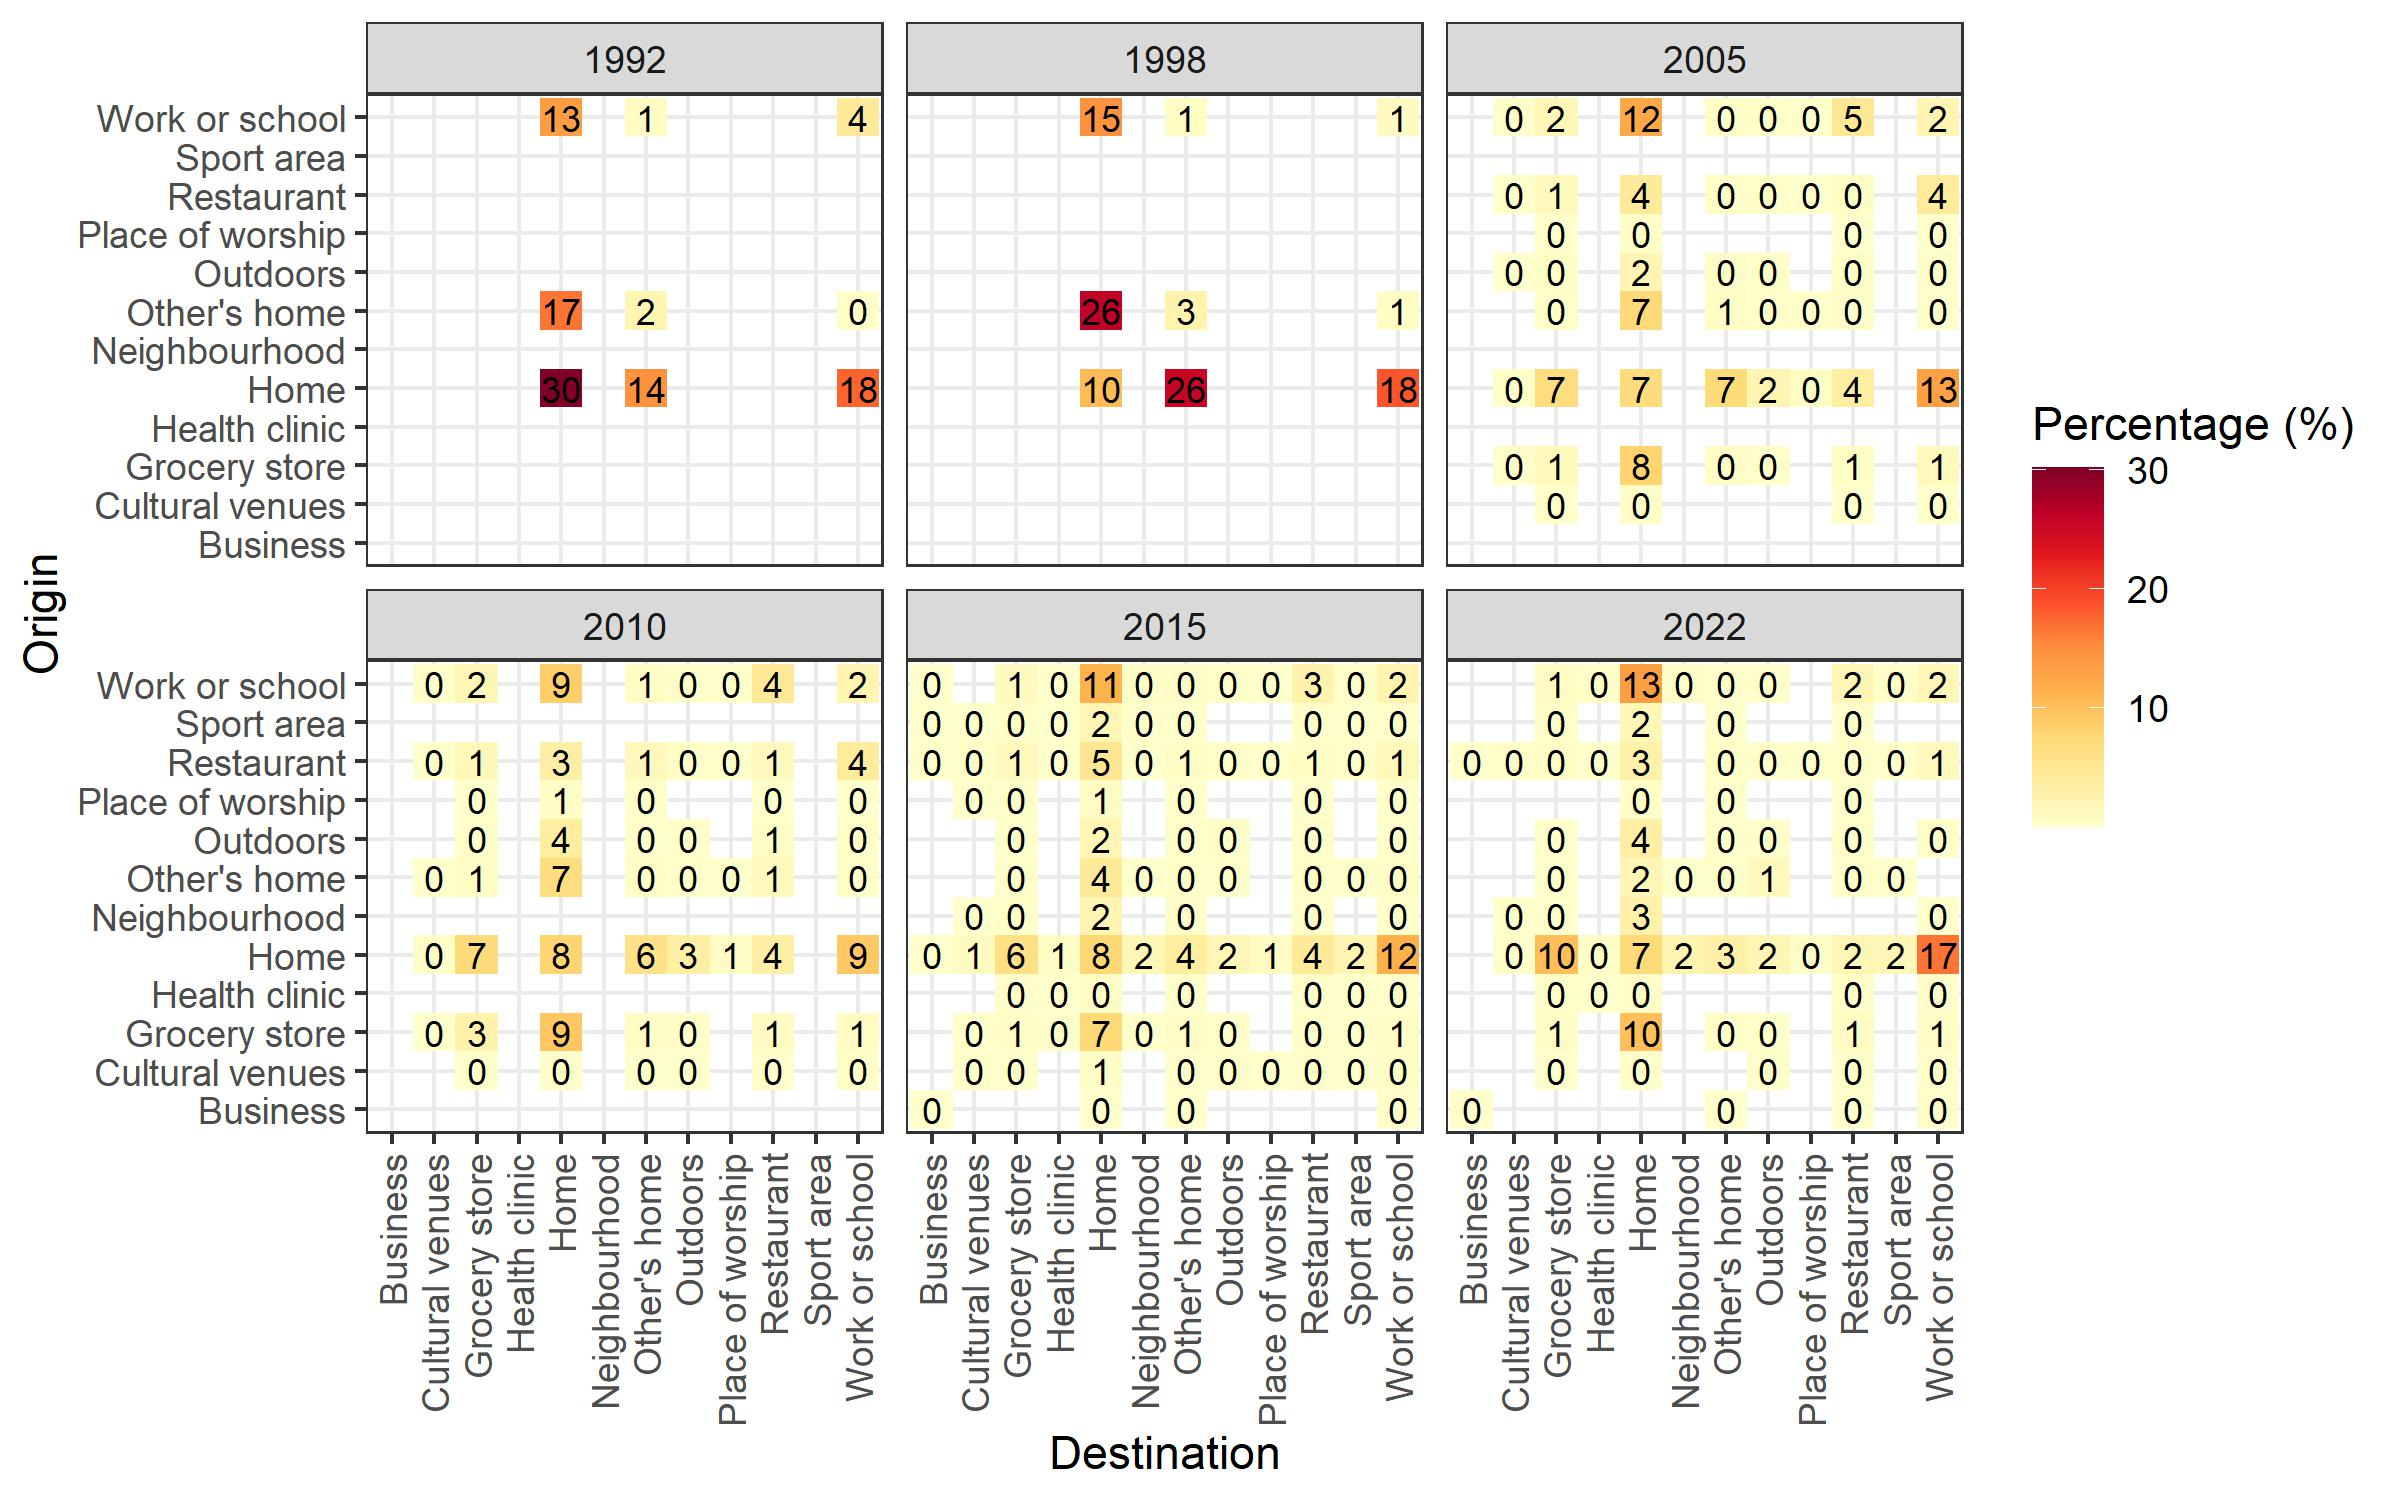
\includegraphics[width=1\linewidth]{figures/walking_hm_fig} \caption{Percentage of walking trips categorized by origin and destination}\label{fig:walking-heatmap}
\end{figure}

\begin{figure}
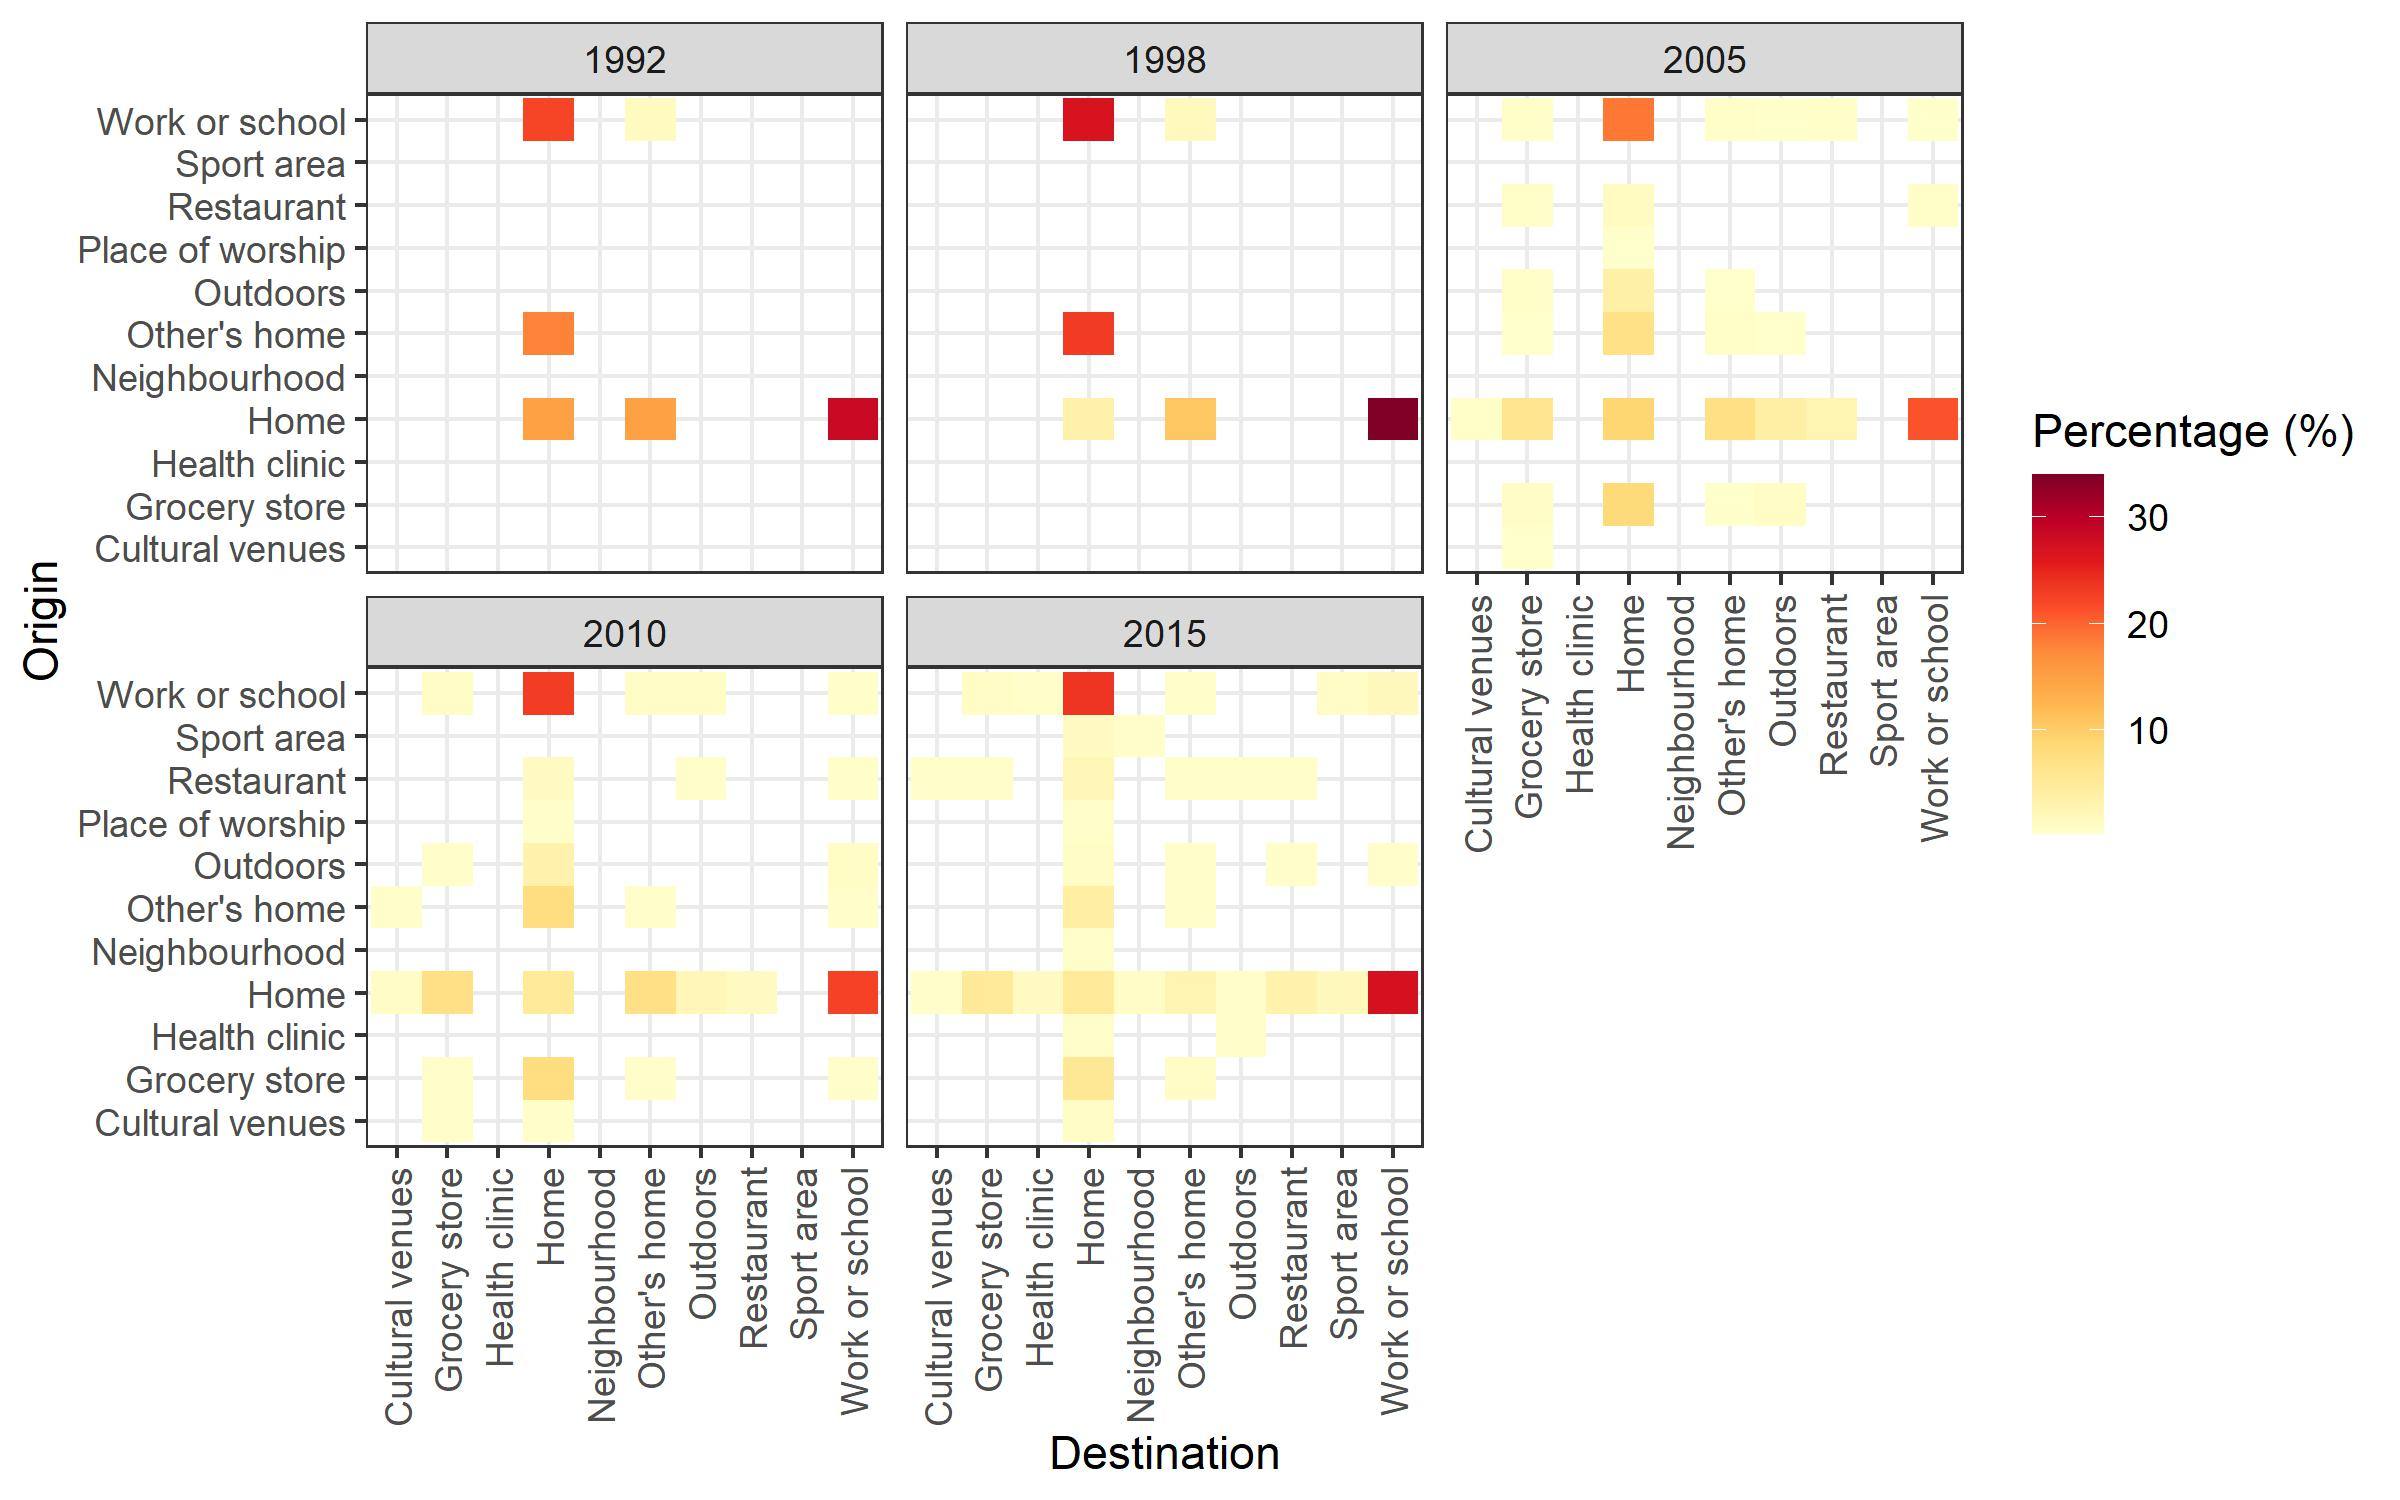
\includegraphics[width=1\linewidth]{figures/cycling_hm_fig} \caption{Percentage of walking trips categorized by origin and destination}\label{fig:cycling-heatmap}
\end{figure}

For cycling trips (Figure \ref{fig:cycling-heatmap}), in 1992, the most
common trip was from ``Home'' to ``Work or school'' (26\%), followed by
trips from ``Other's home'' to ``Home'' (22\%). In all following years,
the most frequent trip were between ``Home'' and ``Work or school'' in
both direction. This combination accounted for 65\% of the trips in
1998, 40\% in 2005, 52\% in 2010, and 58\% in 2015. However, in 2022,
this combination dropped to 43\%, mainly due to an increase in trips
between the ``Grocery store'' and ``Home'' (18\%). Additionally and
unlike walking trips, ``Home'' to ``Home'' trips were not a common
cycling trip in any of the surveys. This suggests that leisure trips,
such as activities around the home, are predominantly done by foot
rather than by bicycle.

We analyzed whether the temporal differences in travel times for the
destinations were statistically significant. Only destinations that
appear in more than one survey year can have their temporal evolution
analyzed. Therefore, out of the twelve possible destinations, some
cycling locations could not be temporally analyzed: ``Business,''
``Neighborhood,'' and ``Place of worship.'' In the case of walking
trips, all destinations could be analyzed over time.

After performing the Kruskal-Wallis test (to assess whether there was a
statistically significant difference between the distributions of
empirical travel time values, considering the time differences for each
destination and the weight of each episode) and the pairwise Wilcoxon
test, we were able to identify the destinations where a statistically
significant difference was detected. For both AT modes, the possible
destinations had at least two year with statistically significant
difference in travel times (p-value \textless{} 0.05, Table A.1).
Considering the cycling mode and, for instance, the ``Home''
destination, there was a statistically significant difference for every
possible combination of two survey cycles. This result indicates that
the previously discussed increase in typical cycling travel time for
home destinations when compared 2022 to 1992 is statistically
significant.

\subsubsection{Population with records of active
trip}\label{population-with-records-of-active-trip}

The share of the population with active trip records varied between
6.93\%, value of 1992, and 15.06\%, value of 2015, from 1992 to 2022
(Table \ref{tab:pop-stats-table}). In 2015, the trend of increasing
participation in walking and cycling trips was reversed to the beginning
of a decline, confirmed by the 2022 survey. In 2015, around 12\% of the
population recorded at least one active trip. In 2022, this share of the
population fell to 9.45\%, the lowest level since 2005, representing
\emph{2,605,395} people out of a total population of \emph{27,584,823}
people.

\begin{landscape}\begingroup\fontsize{10}{12}\selectfont

\begin{longtable}[t]{>{}lrrrrr>{}r|rrrrr>{}r|rrrrrr}
\caption{\label{tab:pop-table-with-prevalence}\label{tab:pop-stats-table}Prevalence of active trip by transportation mode, year of analysis, gender and age group.}\\
\toprule
\multicolumn{1}{c}{ } & \multicolumn{6}{c}{Walking} & \multicolumn{6}{c}{Cycling} & \multicolumn{6}{c}{Both modes} \\
\cmidrule(l{3pt}r{3pt}){2-7} \cmidrule(l{3pt}r{3pt}){8-13} \cmidrule(l{3pt}r{3pt}){14-19}
  & 1992 & 1998 & 2005 & 2010 & 2015 & 2022 & 1992 & 1998 & 2005 & 2010 & 2015 & 2022 & 1992 & 1998 & 2005 & 2010 & 2015 & 2022\\
\midrule
\textbf{Total} & 8.11 & 6.29 & 13.18 & 14.20 & 10.91 & 8.66 & 1.05 & 0.68 & 0.99 & 1.17 & 0.99 & 0.89 & 9.11 & 6.93 & 14.06 & 15.06 & 11.65 & 9.45\\
\textbf{Men+} & 7.53 & 5.03 & 11.90 & 13.93 & 10.85 & 8.89 & 1.45 & 1.18 & 1.56 & 1.87 & 1.34 & 1.33 & 8.94 & 6.18 & 13.31 & 15.31 & 11.89 & 10.05\\
\textbf{Women+} & 8.69 & 7.52 & 14.42 & 14.46 & 10.97 & 8.43 & 0.66 & 0.18 & 0.45 & 0.50 & 0.65 & 0.47 & 9.27 & 7.66 & 14.78 & 14.82 & 11.42 & 8.84\\
\textbf{15 - 24} & 12.48 & 8.38 & 25.01 & 22.28 & 17.33 & 19.88 & 2.50 & 1.16 & 2.08 & 2.75 & 1.06 & 1.58 & 14.97 & 9.30 & 26.88 & 24.01 & 17.91 & 21.47\\
\textbf{25 - 34} & 7.15 & 5.44 & 13.33 & 15.24 & 14.80 & 9.74 & 1.66 & 0.46 & 1.19 & 1.17 & 1.57 & 1.62 & 8.82 & 5.90 & 14.28 & 16.11 & 15.78 & 11.21\\
\addlinespace
\textbf{35 - 44} & 5.79 & 6.40 & 10.52 & 13.46 & 9.38 & 5.23 & 0.65 & 1.14 & 1.01 & 1.06 & 1.17 & 0.83 & 6.24 & 7.54 & 11.43 & 14.34 & 10.50 & 5.78\\
\textbf{45 - 54} & 7.55 & 5.90 & 9.40 & 11.69 & 7.76 & 5.71 & 0.30 & 0.63 & 0.51 & 0.84 & 0.75 & 0.82 & 7.73 & 6.53 & 9.85 & 12.35 & 8.22 & 6.30\\
\textbf{55 - 64} & 8.89 & 5.43 & 9.61 & 10.91 & 7.70 & 5.77 & 0.25 & 0.30 & 0.95 & 0.86 & 0.77 & 0.47 & 9.14 & 5.73 & 10.48 & 11.75 & 8.43 & 6.24\\
\textbf{65 - 74} & 8.55 & 5.27 & 8.76 & 11.59 & 8.77 & 6.66 & 0.00 & 0.00 & 0.22 & 0.42 & 0.70 & 0.33 & 8.55 & 5.27 & 8.98 & 11.82 & 9.36 & 6.96\\
\textbf{75+} & 5.92 & 6.84 & 13.54 & 10.91 & 8.63 & 6.93 & 0.00 & 0.00 & 0.00 & 0.07 & 0.57 & 0.09 & 5.92 & 6.84 & 13.54 & 10.98 & 9.20 & 7.02\\
\bottomrule
\end{longtable}
\endgroup{}
\end{landscape}

Our results show a decrease in the active population since 2010 for both
genders (Figure \ref{fig:gender-perc-figure}). However, the decline was
more pronounced among women+ than men+, leading to a shift in the
historical pattern in which women+ had been the more active gender in
Canada \citep{bryan2009, borhani2024}. Women+ peaked at 14.82\% of the
population with a record of active episodes in 2010 but dropped to the
second-lowest level of 8.84\% in 2022 - only higher than the 7.66\%
recorded in 1998. In contrast, Men+, who also peaked in 2010 with
15.31\% of the population reporting active episodes, declined to 10.05\%
in 2022, thus becoming the gender with the higher share of the active
population.

This result aligns with a trend identified by Borhani et al.
\citeyearpar{borhani2024}. In their study, the authors found that a
higher proportion of females than males reported engaging in any form of
AT, whether walking or cycling, in the last 7 days or 3 months. However,
they also observed that this gender gap appears to have narrowed over
time.

When analyzing by transportation mode, in all survey years a higher
proportion of men+ reported at least one cycling episode on the previous
day compared to women+ (ranging from 1.18\% to 1.87\% for men+ and
0.18\% to 0.66\% for women+). This pattern of more men+ participating in
cycling activities when compared to women+ is consistent with previous
research \citep{heesch2012, bryan2009, borhani2024}. Conversely, women+
historically reported more walking trips than men+, also consistent with
previous research \citep{goel2023, pollard2017, bryan2009, borhani2024},
but this pattern changed in the most recent survey (2022), reinforcing a
trend already present in 2015. In 2022, 8.43\% of women+ reported at
least one walking episode, compared to 8.89\% of Men+.

\begin{figure}
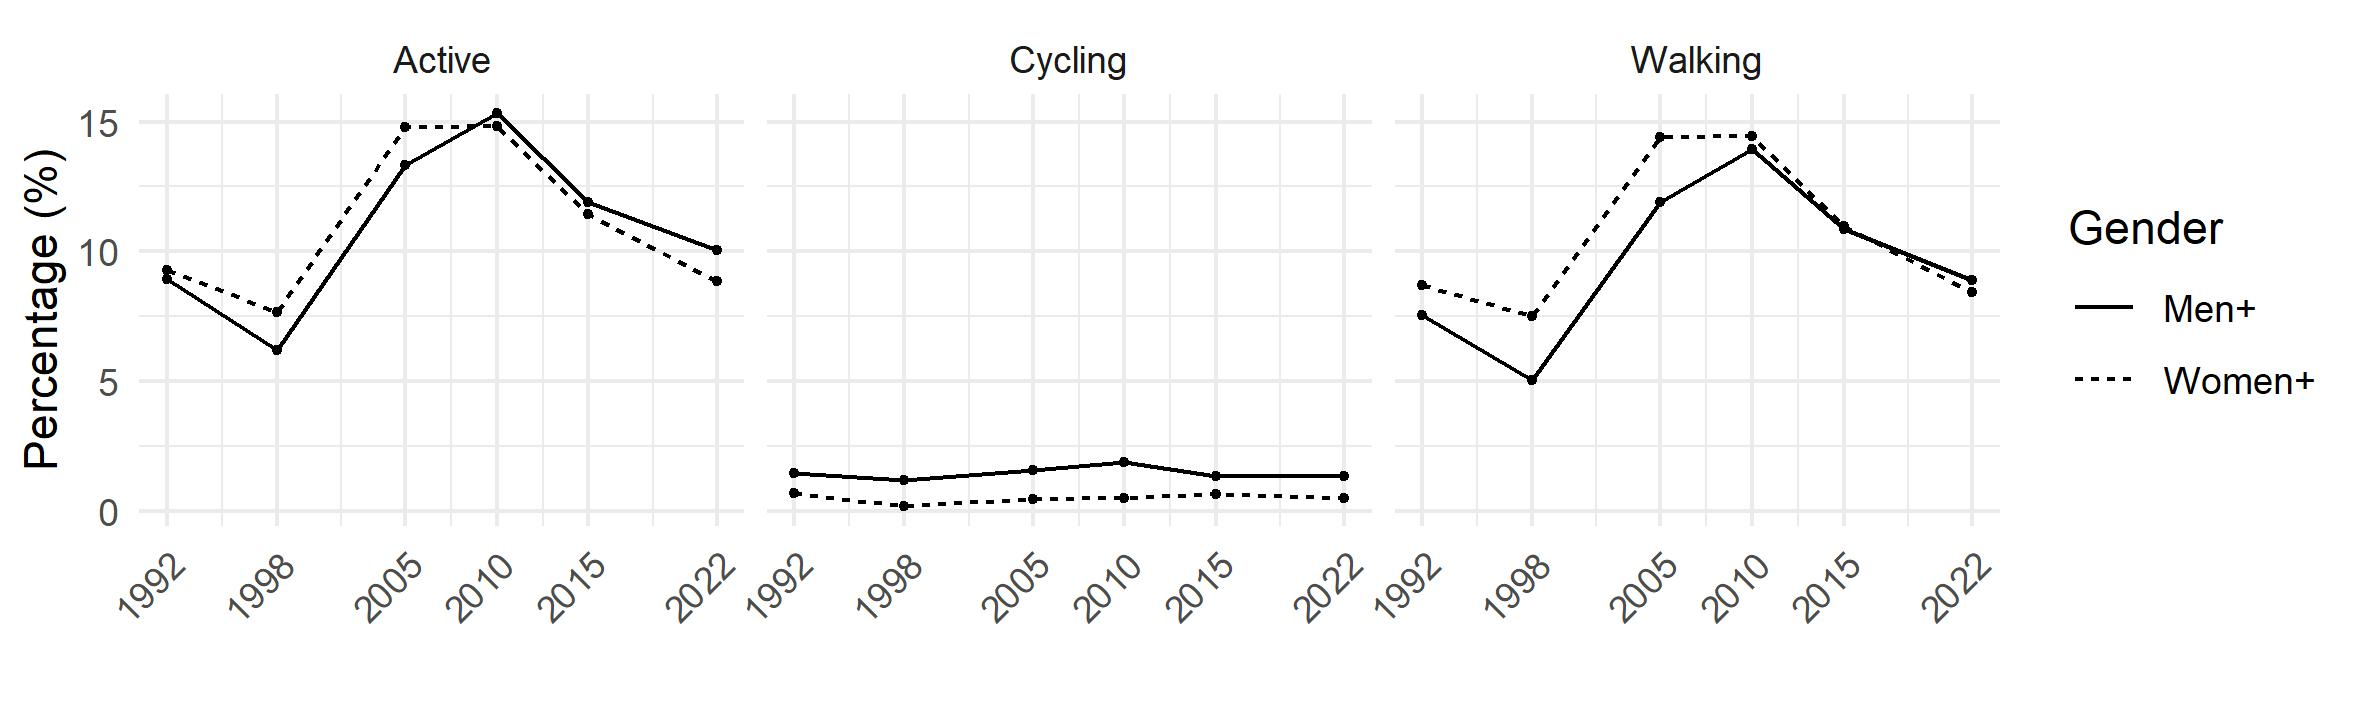
\includegraphics[width=1\linewidth]{figures/active_pop_gender_graph} \caption{Prevelance in activity transportation by gender.}\label{fig:gender-perc-figure}
\end{figure}

When we analyze the population by age group (Figure
\ref{fig:age-perc-figure}), the youngest (those between 15 and 24 years)
stand out as the most active group, ranging from 9.3\% to 26.88\%, and
marking 21.47\% in the most recent survey. This is the only group that
did not show a decrease in the prevalence of active participation over
the last decade, increasing from a low of 17.91\% in 2015 to 21.47\% in
2022 - although still below the levels recorded 2005 (26.88\%). The
survey of 2022 is one more evidence of caracterists of the Generation z
(born between 1997 and 2012) \citep{dimock2019} are noticeably less
dependent on cars and instead use environmentally friendly modes of
travel, such as public transport, cycling and walking, more often than
not \citep{haseeb2024, grimsrud2014, kuhnimhof2011}. Historically, and
in consistency with the literature \citep{bryan2009, borhani2024},
prevalence decreases as age increases. However, in the most recent
survey (2022), as well as in 2005, the oldest group (75 years and older)
presented the third-highest prevalence (7.02\%), surpassing younger
groups.

The analysis by mode shows a similar trend (Figure
\ref{fig:age-perc-figure}). However, for cycling, the second youngest
group (aged 25 to 34 years) had the highest prevalence in the 2022
survey (1.62\%), surpassing the youngest group (1.58\%). For all other
age groups, cycling prevalence decreases as age increases, approaching
0.10\% for the oldest group (75 years and older).

\begin{figure}
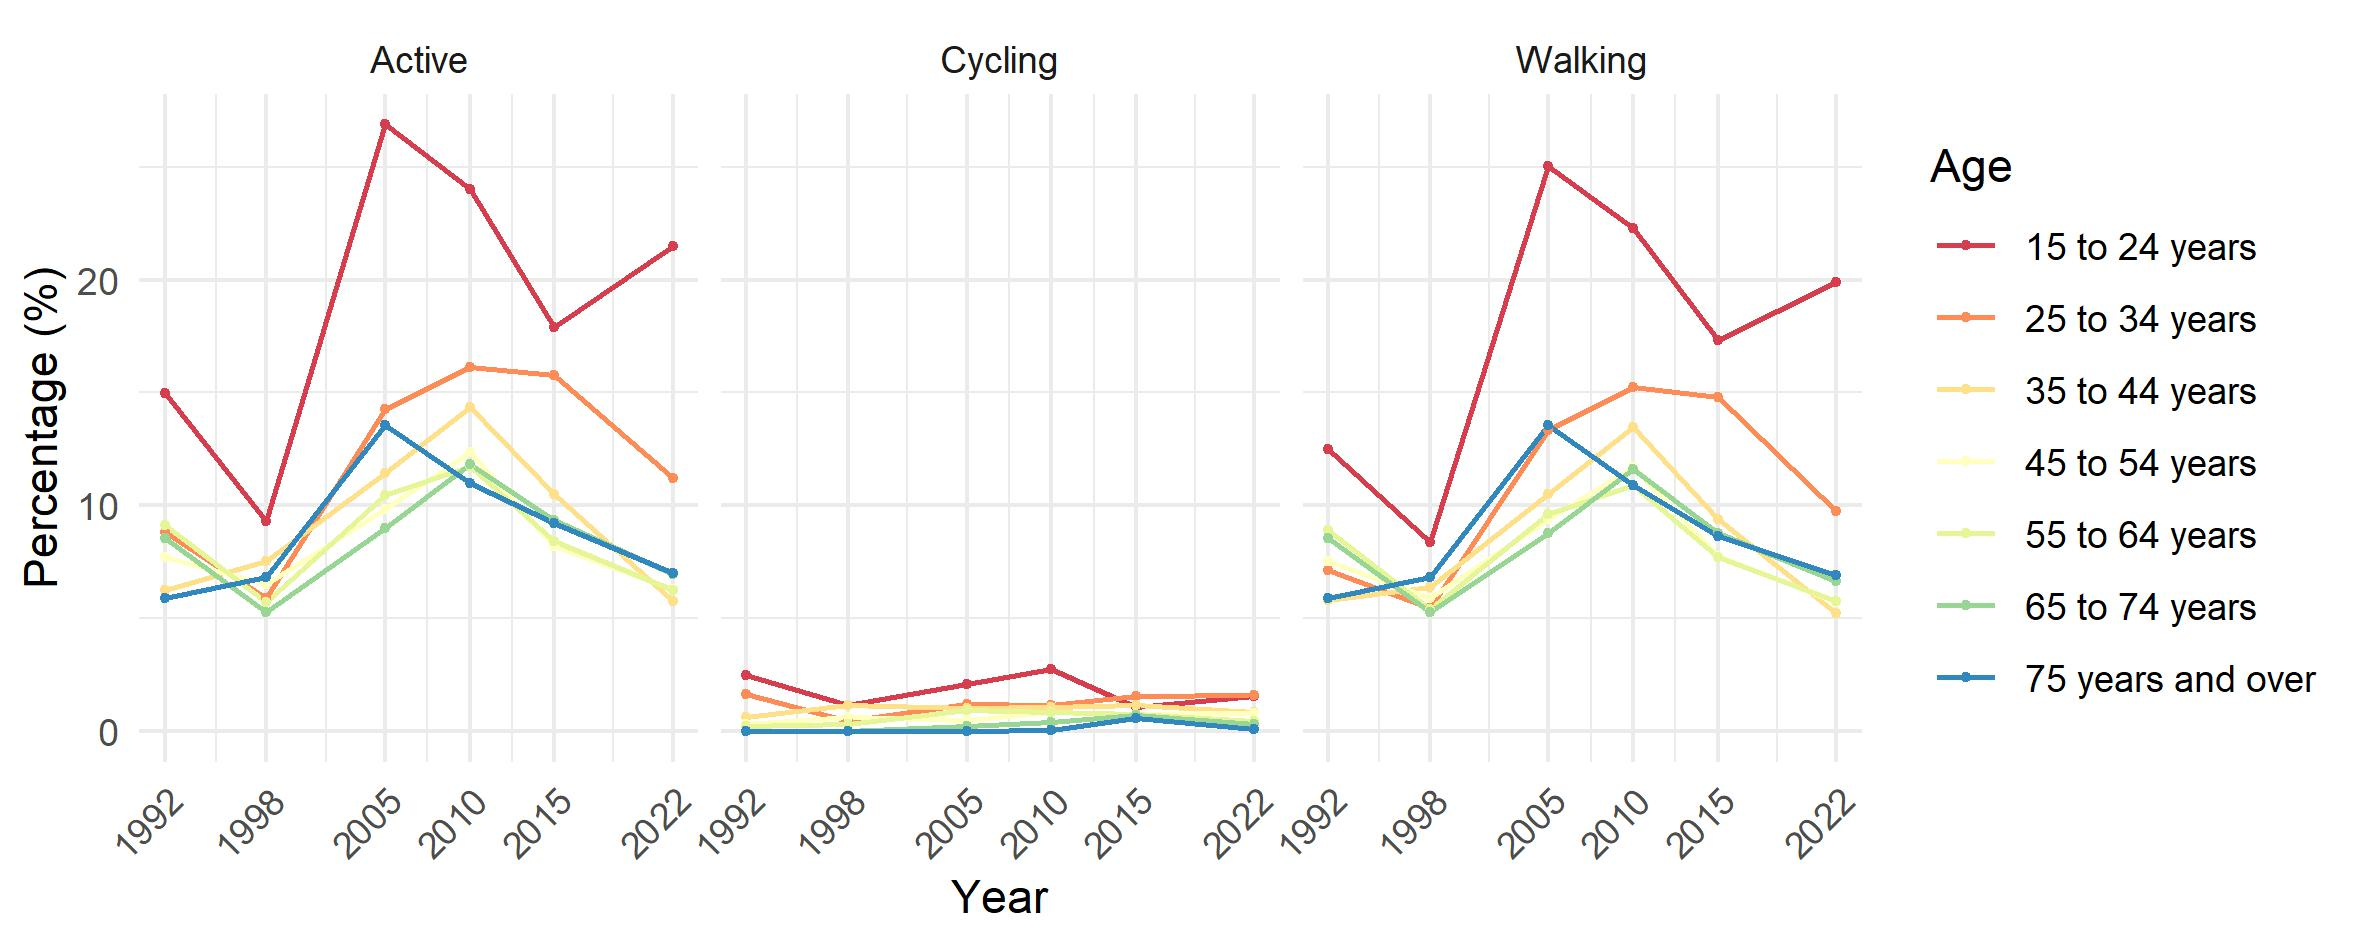
\includegraphics[width=1\linewidth]{figures/active_pop_age_graph} \caption{Prevelance in activity transportation by age group.}\label{fig:age-perc-figure}
\end{figure}

The number of people with active trip episodes is mainly influenced by
walking episodes, since over 90\% of the recorded active trips involve
individuals with walking episodes. Analyzing the number of episodes per
person with records of AT, the average is around 1.96 active episodes
per person, varying from a maximum of 2.10 episodes in 2005 to a minimum
of 1.72 episodes per person in 1992. Figure \ref{fig:gender-eps-figure}
presents, for each survey year, the total number of active episodes
divided by the population with active records, the number of walking
episodes per person who walked, and the number of cycling episodes per
person who cycled - all disaggregated by gender. Until 2022, men+
historically had more number of active episodes when compared to women+,
but this pattern changed in the last survey when men+ scored 2.07 active
episodes, when compared to 2.11 active episodes made by women+. This was
mainly caused by the decreasing of number of walking episodes made by
men+ (from 2.16 to 2.07 from 2015 to 2022), and increase of walking
episodes made by women+ (from 1.92 to 2.11 in the same period).

\begin{figure}
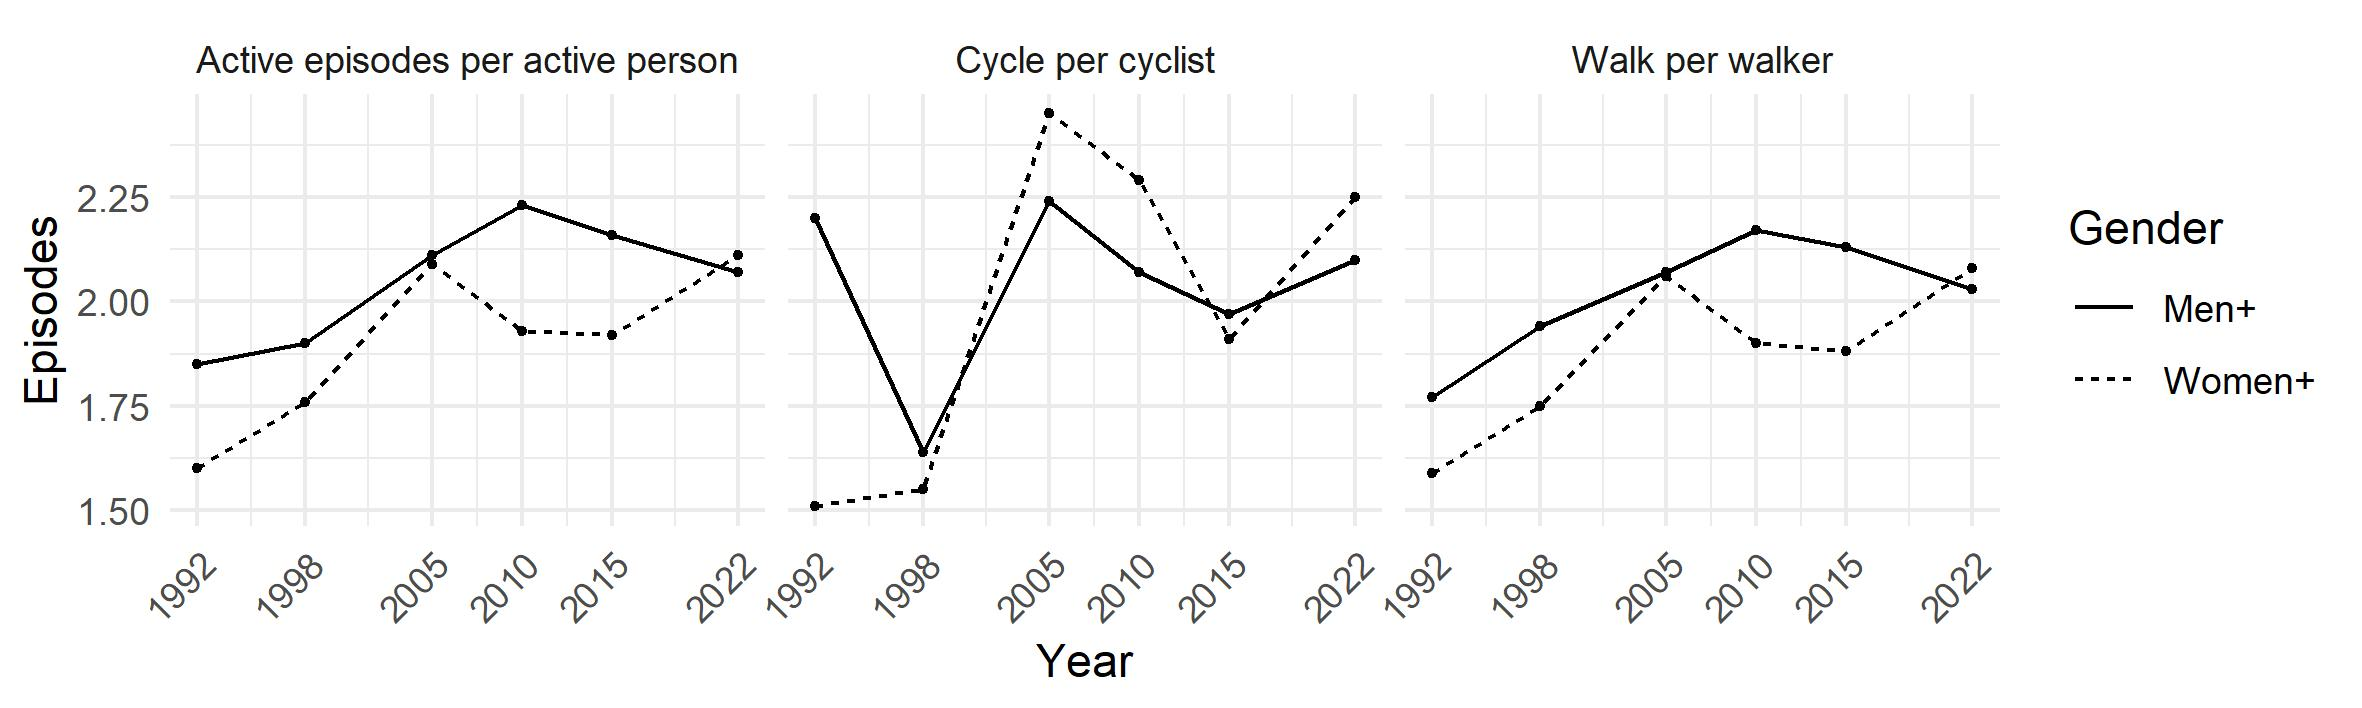
\includegraphics[width=1\linewidth]{figures/eps_gender_graph} \caption{Episodes per active person by gender.}\label{fig:gender-eps-figure}
\end{figure}

The same type of metric shown in Figure \ref{fig:gender-eps-figure} can
also be calculated by age group. Figure \ref{fig:age-eps-figure} shows
that active individuals in the oldest age group (those aged 75 and over)
have been on an increasing trend in the number of active episodes since
2010. In 2010, this group ranked last in the number of active episodes
per active person (1.94), and by 2022, it had taken first place with
2.21 episodes per active person (a 14\% increase). In general, all age
groups have improved their performance compared to 1992. However, over a
shorter period between the two most recent surveys (2015 and 2022), the
group aged 25 to 34 is the only one that showed a decrease in the number
of active episodes per active person, decreasing from 2.27 to 1.93
episodes (15\% of reduction).

When the age group analysis is split by transportation mode, walking
episodes per walker follow a pattern similar to that of total active
episodes per active person (Figure \ref{fig:age-eps-figure}). However,
the pattern for cycling differs. For almost every age group, the data
can be divided into two distinct time periods: before and after 2005.
From 1992 to 2005, there was a general trend of increasing cycling
episodes per cyclist (from 1.72 to 2.10). This trend is exemplified by
the 55 to 64 age group, which increased from 1.58 to 2.61 episodes (a
65\% rise). This period was followed by a decline in cycling episodes
per cyclist from 2005 to 2022 (from 2.10 to 2.04). A clear example of
this trend is the 65 to 74 age group, which saw a decrease from 2.73 to
1.60 episodes (a reduction of 41\%). In more recent years, only two age
groups show an increasing trend in cycling episodes per cyclist when
comparing the last two surveys (2015 and 2022): the youngest group (15
to 24 years) and the oldest (75 and over). In both cases, there was a
significant increase. The youngest group rose from 1.78 to 3.00 episodes
(a 40\% increase), while the oldest group doubled its average from 1.00
to 2.00 episodes over the seven years.

\begin{figure}
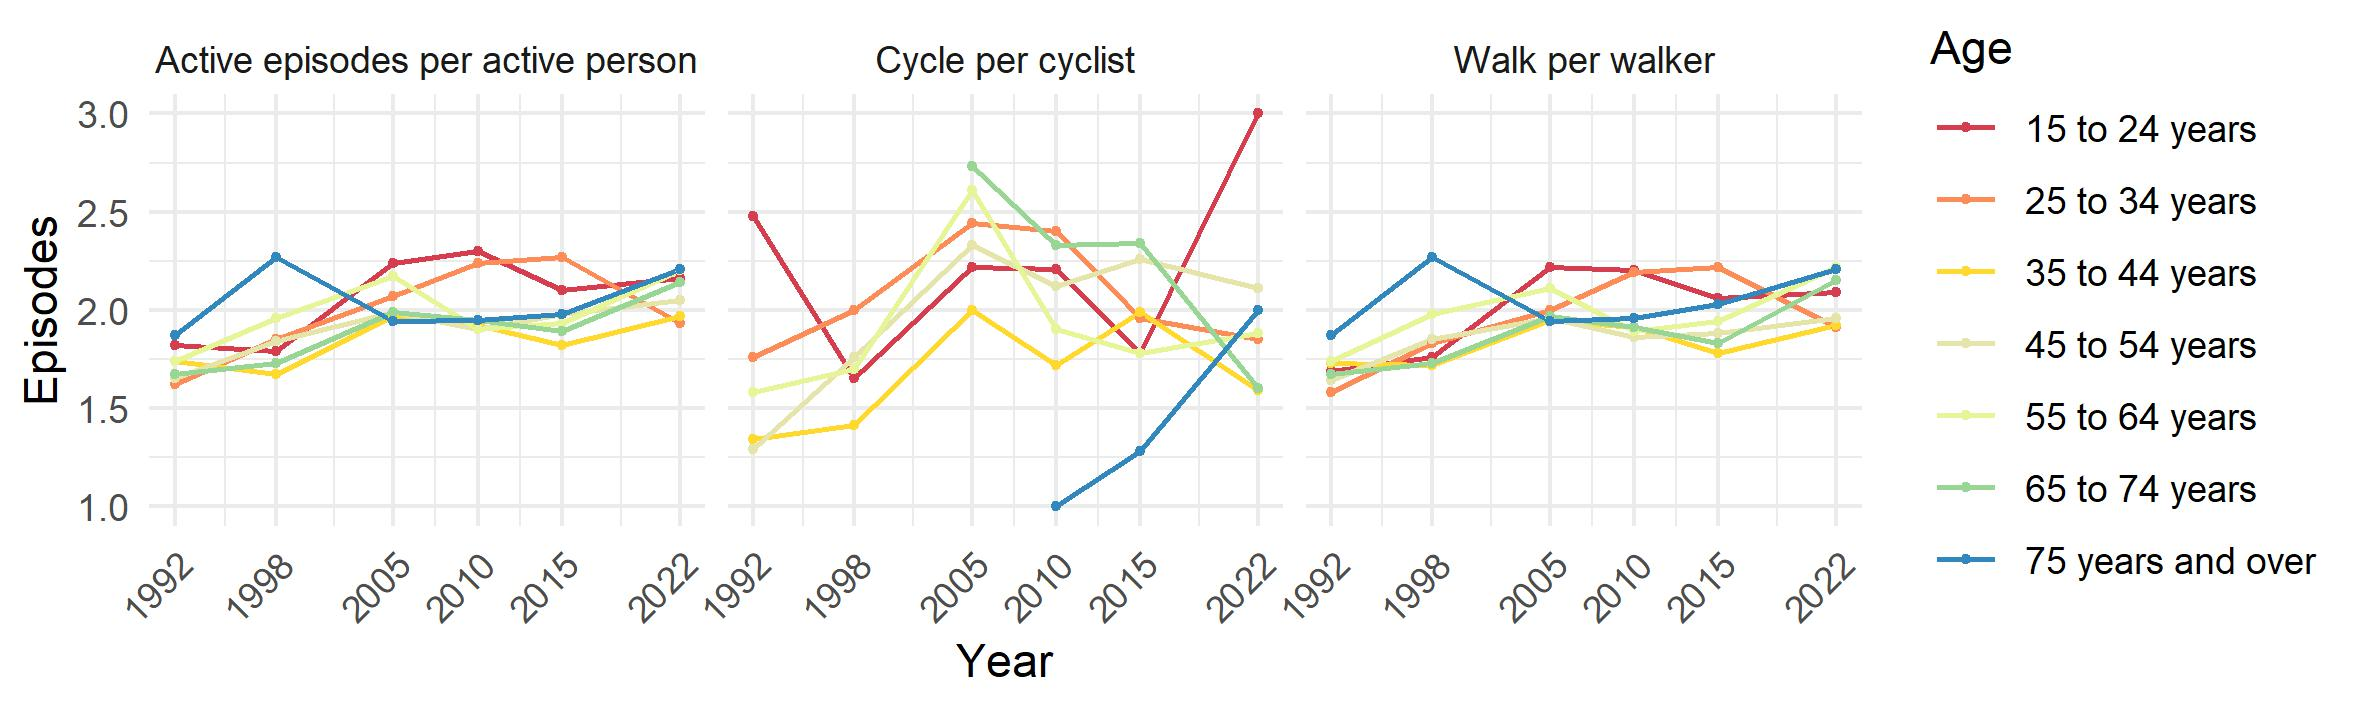
\includegraphics[width=1\linewidth]{figures/eps_age_graph} \caption{Episodes per active person by age group.}\label{fig:age-eps-figure}
\end{figure}

Regarding the duration of the AT episodes, we observe an increase in the
typical duration of active travel for both genders and both
transportation modes after 2010 (Figure \ref{fig:gender-dur-figure}),
without gender difference in general AT. The median remained stable at
10 minutes for both men+ and women+ from 2005 to 2015, increasing to 15
minutes in 2022. However, for cycling trips, the median cycling duration
shows a clear gender difference: men+ reported a median of 30 minutes in
2022, up from 15 minutes in 2005. This represents the highest median
duration recorded across the entire historical series. In contrast,
women+ tended to maintain a median duration around 15 minutes, which was
also the value reported in the most recent survey.

\begin{figure}
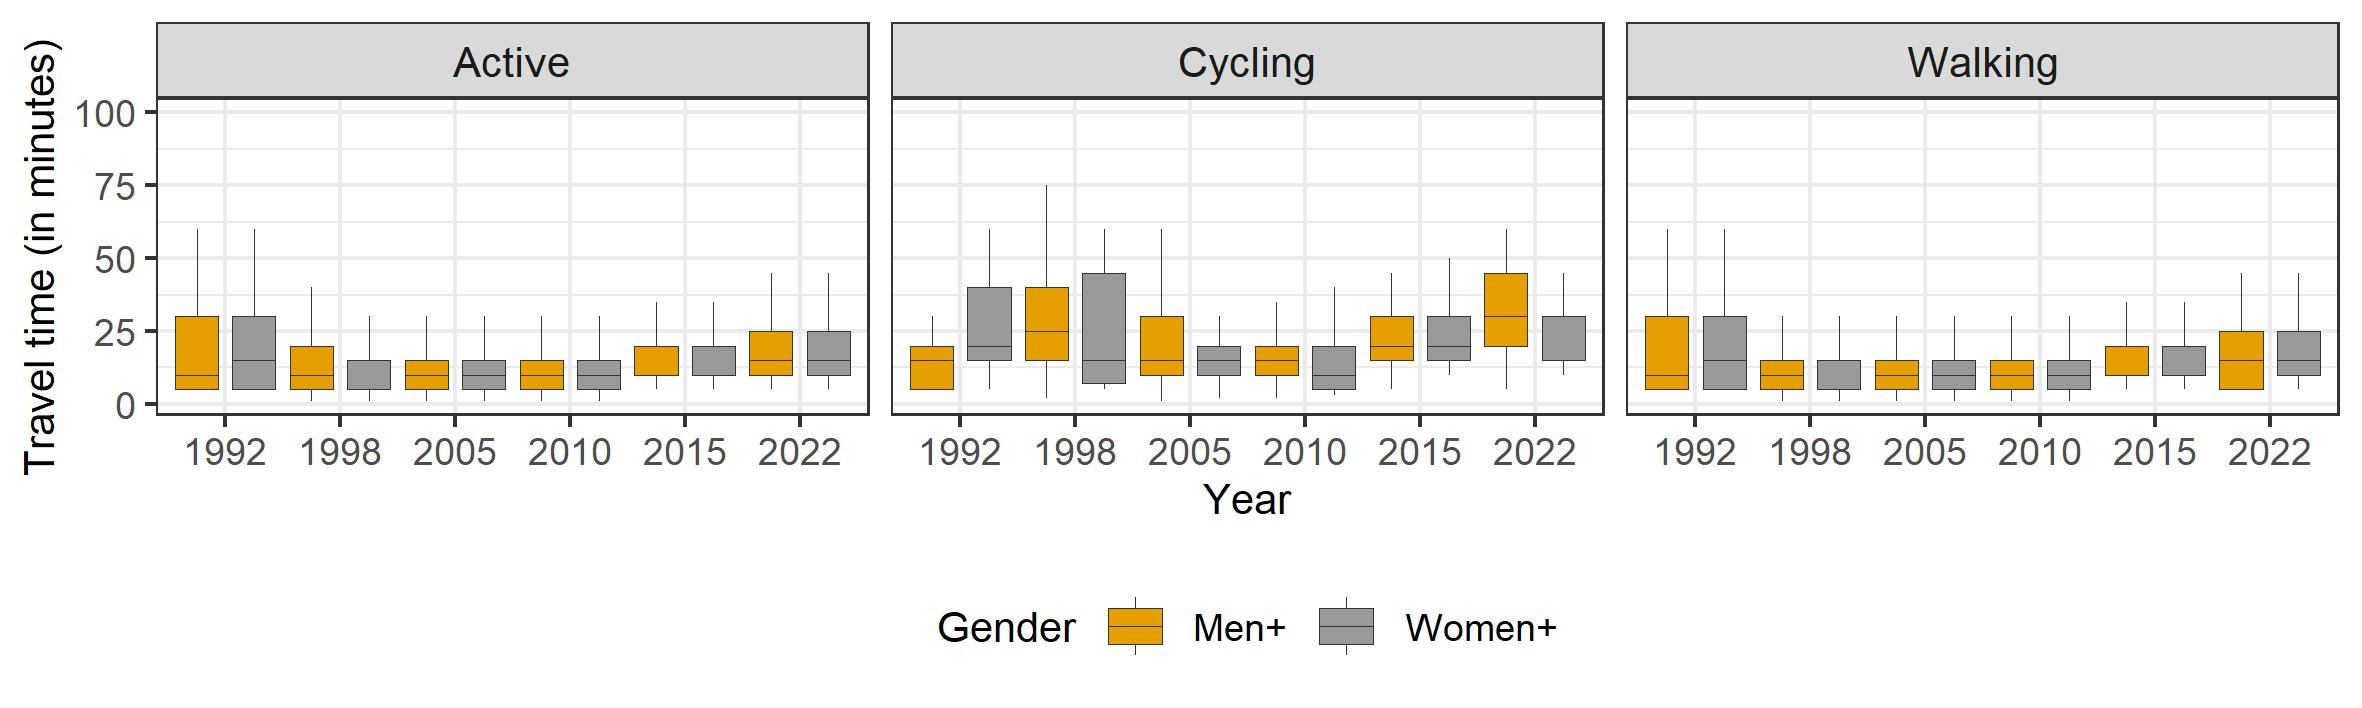
\includegraphics[width=1\linewidth]{figures/gender_duration_boxplots} \caption{Duration (in minutes) of active episodes by gender.}\label{fig:gender-dur-figure}
\end{figure}

An examination of typical trip length by age group reveals a general
increase in AT trip duration across all groups since 1998 (Figure
\ref{fig:age-dur-figure}). With the exception of the 65 to 74 age group,
where the average duration has remained at 10 minutes, all other groups
have increased to a typical duration of 15 minutes. Regarding median
values, the typical trip duration was 25 minutes for most groups, except
for the 35 to 54 age group, which recorded a median of 20 minutes, and
the 65 to 74 group, which recorded a median of 60 minutes.

\begin{figure}
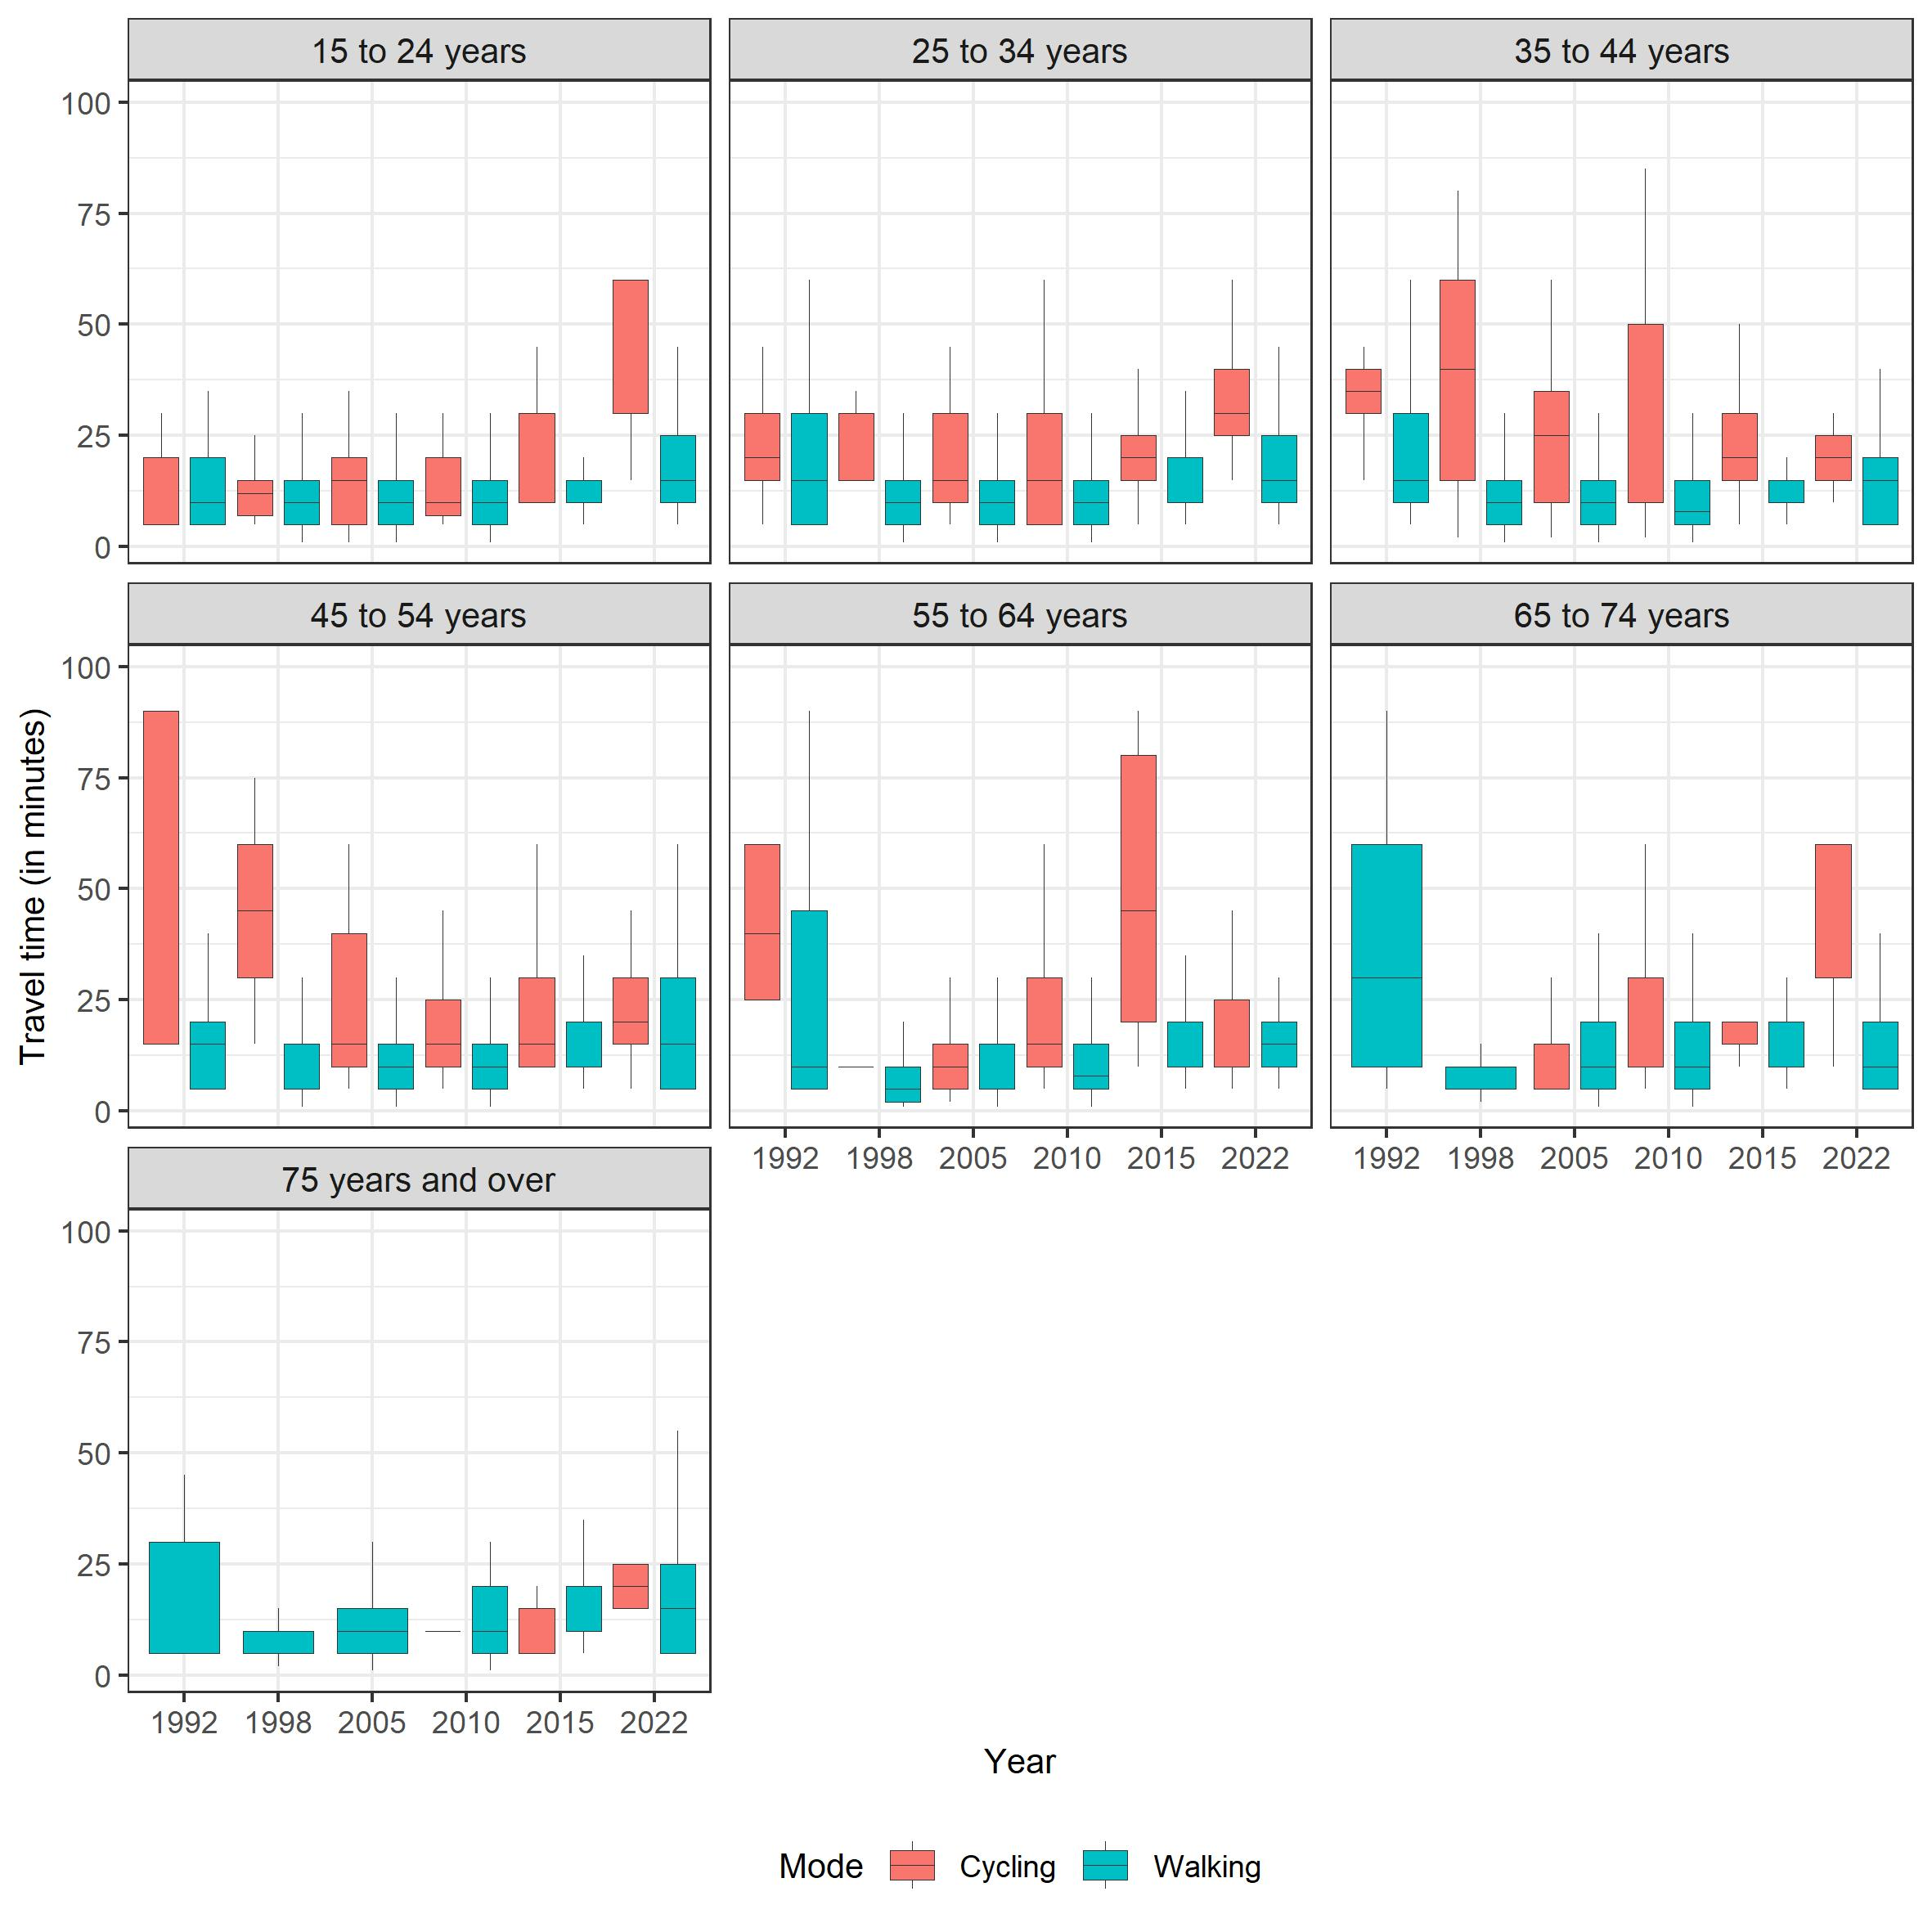
\includegraphics[width=1\linewidth]{figures/age_duration_boxplots} \caption{Duration (in minutes) of active episodes by Age group.}\label{fig:age-dur-figure}
\end{figure}

\subsection{Calibrated impedance
function}\label{calibrated-impedance-function}

After analyzing the active travel episodes and population with records
of active trip, this section presents the identified impedance functions
for walking and cycling trips to various destinations across CMA/CA in
Canada from 1992 to 2022. In general, the impedance functions aim to
capture transportation behavior, illustrating that the likelihood of
traveling between two points decreases as travel duration increases.
Each impedance function follows one of the mathematical equations
previously mentioned, enabling the plotting of PDF curves. These curves
also highlight critical points at which a person's tendency to walk or
cycle significantly decreases.

As explained in the methodology section, we used the
\texttt{fitdistrplus} package \citep{delignette2015fitdistrplus} to
calibrate the functions. We selected the best impedance function for
each transportation mode, destination, and year based on the lowest
Akaike Information Criterion (AIC) value \citep{akaike1974}. The AIC
metric not only assesses the goodness of fit but also penalizes model
complexity to prevent overfitting. AIC provides a balance between a
model's accuracy and simplicity, with lower values indicating a more
economical model. The distribution with the lowest AIC was considered
the most suitable for representing the distance decay curve for each
specific destination in each year. We chose AIC as the selection
criterion because, while the \texttt{fitdistrplus} package accommodates
weighted episodes during estimation, it does not extend this
functionality to diagnostic plots, which are typically unweighted and
traditionally used to select the best-fitting function.

In total, we fitted 83 impedance functions. Among the candidate
distributions, only the negative exponential type was not selected. The
absence of exponential functions, given the variety of destinations,
year and mode of transport, indicates that the impedance functions
applied in active accessibility studies may not be adequately measuring
travel behavior, especially for cases when the travel time is close to 0
minute. Table \ref{tab:walking-functions-tab} displays the selected
functions for walking trips, while Table \ref{tab:cycling-functions-tab}
presents the functions for cycling trips.

\begin{table}
\centering
\caption{\label{tab:selected-functions}\label{tab:walking-functions-tab}Impedance functions and AIC for walking trips.}
\centering
\resizebox{\ifdim\width>\linewidth\linewidth\else\width\fi}{!}{
\fontsize{8}{10}\selectfont
\begin{threeparttable}
\begin{tabular}[t]{rllrrrr}
\toprule
\multicolumn{1}{c}{\textbf{Year}} & \multicolumn{1}{c}{\textbf{Destination}} & \multicolumn{1}{c}{\textbf{Impedance function}} & \multicolumn{1}{c}{\textbf{Parameter 1*}} & \multicolumn{1}{c}{\textbf{Parameter 2*}} & \multicolumn{1}{c}{\textbf{AIC}} & \multicolumn{1}{c}{\textbf{Count}}\\
\midrule
 & Home & Lognormal & 2.92 & 0.77 & 7761103 & 296\\

 & Other's home & Lognormal & 2.15 & 0.84 & 1778150 & 81\\

\multirow[t]{-3}{*}{\raggedleft\arraybackslash 1992} & Work or school & Lognormal & 2.38 & 0.70 & 2319400 & 113\\
\cmidrule{1-7}
 & Home & Lognormal & 2.07 & 0.92 & 5656275 & 302\\

 & Other's home & Lognormal & 1.75 & 0.97 & 2892771 & 176\\

\multirow[t]{-3}{*}{\raggedleft\arraybackslash 1998} & Work or school & Gamma & 1.23 & 0.09 & 2318752 & 109\\
\cmidrule{1-7}
 & Cultural venues & Gamma & 4.10 & 0.34 & 238506 & 25\\

 & Grocery store & Gamma & 1.22 & 0.10 & 4776215 & 558\\

 & Home & Gamma & 1.16 & 0.08 & 17291041 & 1831\\

 & Other's home & Gamma & 1.03 & 0.11 & 3420742 & 436\\

 & Outdoors & Gamma & 1.24 & 0.13 & 1272012 & 155\\

 & Place of worship & Gamma & 2.07 & 0.19 & 228307 & 32\\

 & Restaurant & Lognormal & 1.95 & 0.79 & 3727576 & 421\\

\multirow[t]{-8}{*}{\raggedleft\arraybackslash 2005} & Work or school & Lognormal & 2.13 & 0.79 & 8182691 & 724\\
\cmidrule{1-7}
 & Cultural venues & Gamma & 3.60 & 0.34 & 304141 & 25\\

 & Grocery store & Lognormal & 2.08 & 0.85 & 6369652 & 489\\

 & Home & Gamma & 1.10 & 0.07 & 19584386 & 1424\\

 & Other's home & Lognormal & 1.81 & 0.92 & 4035574 & 336\\

 & Outdoors & Gamma & 1.27 & 0.13 & 2114346 & 167\\

 & Place of worship & Lognormal & 1.95 & 0.70 & 285177 & 28\\

 & Restaurant & Lognormal & 2.01 & 0.90 & 5187191 & 371\\

\multirow[t]{-8}{*}{\raggedleft\arraybackslash 2010} & Work or school & Lognormal & 2.21 & 0.78 & 7917431 & 494\\
\cmidrule{1-7}
 & Business & Lognormal & 2.41 & 0.67 & 102286 & 8\\

 & Cultural venues & Gamma & 4.57 & 0.34 & 543242 & 43\\

 & Grocery store & Lognormal & 2.48 & 0.68 & 4001111 & 338\\

 & Health clinic & Lognormal & 2.44 & 0.70 & 324578 & 27\\

 & Home & Lognormal & 2.57 & 0.74 & 17235960 & 1202\\

 & Neighbourhood & Lognormal & 2.41 & 0.77 & 981626 & 53\\

 & Other's home & Lognormal & 2.43 & 0.80 & 2388598 & 186\\

 & Outdoors & Lognormal & 2.54 & 0.79 & 1247963 & 72\\

 & Place of worship & Gamma & 5.64 & 0.28 & 343187 & 24\\

 & Restaurant & Lognormal & 2.38 & 0.74 & 3490082 & 231\\

 & Sport area & Lognormal & 2.48 & 0.59 & 1199687 & 94\\

\multirow[t]{-12}{*}{\raggedleft\arraybackslash 2015} & Work or school & Lognormal & 2.55 & 0.64 & 6612061 & 407\\
\cmidrule{1-7}
 & Business & Uniform & 0.00 & 20.97 & 56268 & 5\\

 & Cultural venues & Gamma & 3.89 & 0.24 & 157354 & 12\\

 & Grocery store & Lognormal & 2.78 & 0.62 & 4618945 & 192\\

 & Health clinic & Lognormal & 2.40 & 0.98 & 325649 & 12\\

 & Home & Lognormal & 2.80 & 0.67 & 16787347 & 633\\

 & Neighbourhood & Lognormal & 2.28 & 0.88 & 963957 & 33\\

 & Other's home & Lognormal & 2.23 & 0.80 & 1463414 & 86\\

 & Outdoors & Lognormal & 2.27 & 0.77 & 1313257 & 43\\

 & Place of worship & Uniform & 0.00 & 33.68 & 160837 & 11\\

 & Restaurant & Lognormal & 2.37 & 0.70 & 2098269 & 100\\

 & Sport area & Lognormal & 2.63 & 0.45 & 651353 & 39\\

\multirow[t]{-12}{*}{\raggedleft\arraybackslash 2022} & Work or school & Lognormal & 2.64 & 0.63 & 7432435 & 192\\
\bottomrule
\end{tabular}
\begin{tablenotes}
\item \textit{Note: } 
\item For lognormal distributions, 'Parameter 1' and 'Parameter 2' refer to the mean and standard deviation of the distribution on the logarithmic scaler, respectively. For Gamma distributions, 'Parameter 1' and 'Parameter 2' refer to the rate and shape of the distribution, respectively. For uniform distributions,  'Parameter 1' refers to the minimum lower bound and 'Parameter 2'  refers to the upper bound (maximum) of the distribution.  'AIC' means Akaike information criterion.
\end{tablenotes}
\end{threeparttable}}
\end{table}

\begin{table}
\centering
\caption{\label{tab:selected-functions}\label{tab:cycling-functions-tab}Impedance functions and AIC for cycling trips.}
\centering
\resizebox{\ifdim\width>\linewidth\linewidth\else\width\fi}{!}{
\fontsize{8}{10}\selectfont
\begin{threeparttable}
\begin{tabular}[t]{rllrrrr}
\toprule
\multicolumn{1}{c}{\textbf{Year}} & \multicolumn{1}{c}{\textbf{Destination}} & \multicolumn{1}{c}{\textbf{Impedance function}} & \multicolumn{1}{c}{\textbf{Parameter 1*}} & \multicolumn{1}{c}{\textbf{Parameter 2*}} & \multicolumn{1}{c}{\textbf{AIC}} & \multicolumn{1}{c}{\textbf{Count}}\\
\midrule
 & Home & Gamma & 1.18 & 0.05 & 1018747 & 37\\

 & Other's home & Lognormal & 2.57 & 0.82 & 373451 & 11\\

\multirow[t]{-3}{*}{\raggedleft\arraybackslash 1992} & Work or school & Gamma & 3.00 & 0.17 & 433582 & 19\\
\cmidrule{1-7}
 & Home & Gamma & 1.70 & 0.07 & 715802 & 30\\

 & Other's home & Lognormal & 2.79 & 0.80 & 113905 & 7\\

\multirow[t]{-3}{*}{\raggedleft\arraybackslash 1998} & Work or school & Gamma & 3.37 & 0.10 & 481536 & 19\\
\cmidrule{1-7}
 & Cultural venues & Uniform & 0.00 & 15.13 & 6355 & 2\\

 & Grocery store & Gamma & 1.93 & 0.14 & 320218 & 29\\

 & Home & Gamma & 1.49 & 0.07 & 1794317 & 140\\

 & Other's home & Gamma & 1.84 & 0.15 & 310058 & 27\\

 & Outdoors & Gamma & 2.99 & 0.17 & 215894 & 17\\

 & Restaurant & Gamma & 3.37 & 0.21 & 109072 & 10\\

\multirow[t]{-7}{*}{\raggedleft\arraybackslash 2005} & Work or school & Lognormal & 2.93 & 0.70 & 888655 & 64\\
\cmidrule{1-7}
 & Cultural venues & Uniform & 0.00 & 32.58 & 38938 & 3\\

 & Grocery store & Lognormal & 2.68 & 0.61 & 315037 & 20\\

 & Home & Lognormal & 2.60 & 0.77 & 2006242 & 103\\

 & Other's home & Lognormal & 2.40 & 0.63 & 338777 & 19\\

 & Outdoors & Lognormal & 2.05 & 0.59 & 92699 & 8\\

 & Restaurant & Uniform & 0.00 & 17.49 & 35370 & 3\\

\multirow[t]{-7}{*}{\raggedleft\arraybackslash 2010} & Work or school & Lognormal & 2.65 & 0.77 & 1292760 & 53\\
\cmidrule{1-7}
 & Cultural venues & Lognormal & 2.71 & 0.00 & -Inf & 2\\

 & Grocery store & Lognormal & 3.08 & 0.80 & 229413 & 14\\

 & Health clinic & Lognormal & 2.93 & 0.86 & 80810 & 4\\

 & Home & Lognormal & 3.08 & 0.61 & 1745846 & 98\\

 & Neighbourhood & Uniform & 0.00 & 48.55 & 49924 & 3\\

 & Other's home & Lognormal & 2.52 & 0.44 & 140210 & 12\\

 & Outdoors & Uniform & 0.00 & 35.03 & 31463 & 3\\

 & Restaurant & Lognormal & 3.11 & 0.60 & 115406 & 9\\

 & Sport area & Uniform & 0.00 & 17.47 & 32969 & 6\\

\multirow[t]{-10}{*}{\raggedleft\arraybackslash 2015} & Work or school & Lognormal & 3.03 & 0.41 & 1162876 & 63\\
\cmidrule{1-7}
 & Grocery store & Normal & 47.03 & 20.72 & 602645 & 8\\

 & Health clinic & Uniform & 0.00 & 61.98 & 123138 & 3\\

 & Home & Gamma & 4.04 & 0.15 & 1798770 & 56\\

 & Outdoors & Lognormal & 3.44 & 0.11 & 94804 & 2\\

 & Restaurant & Normal & 26.29 & 5.83 & 100585 & 3\\

 & Sport area & Normal & 29.89 & 17.05 & 124824 & 5\\

\multirow[t]{-7}{*}{\raggedleft\arraybackslash 2022} & Work or school & Gamma & 5.87 & 0.24 & 832953 & 37\\
\bottomrule
\end{tabular}
\begin{tablenotes}
\item \textit{Note: } 
\item For lognormal distributions, 'Parameter 1' and 'Parameter 2' refer to the mean and standard deviation of the distribution on the logarithmic scaler, respectively. For normal distributions, 'Parameter 1' and 'Parameter 2' refer to the mean and standard deviation of the distribution, respectively. For the gamma distributions, 'Parameter 1' and 'Parameter 2' refer to the rate and shape of the distribution, respectively. For the uniform distribution,  'Parameter 1' refers to the minimum lower bound and 'Parameter 2'  refers to the upper bound (maximum) of the distribution.  'AIC' means Akaike information criterion.
\end{tablenotes}
\end{threeparttable}}
\end{table}

Figure \ref{fig:outdoors-impedance-fig} presents the calibrated
functions for the destination `Outdoors,' along with a histogram of the
empirical distribution of trips, split by year and transportation mode.
Comparing functions from different categories can be difficult when
analyzed for the first time, but by starting with the functions from the
walking transportation mode (blue curves), the calibrated functions from
this example show a similar pattern. At a duration of around zero
minutes, the probability of making the trip is lower (with a density of
zero for the years 2015 and 2022). After a few minutes, there is a peak
in the maximum probability of traveling to reach `Outdoors,' followed by
a drop in willingness to zero for very high values of time, indicating a
low probability of making the trip.

\begin{figure}

{\centering 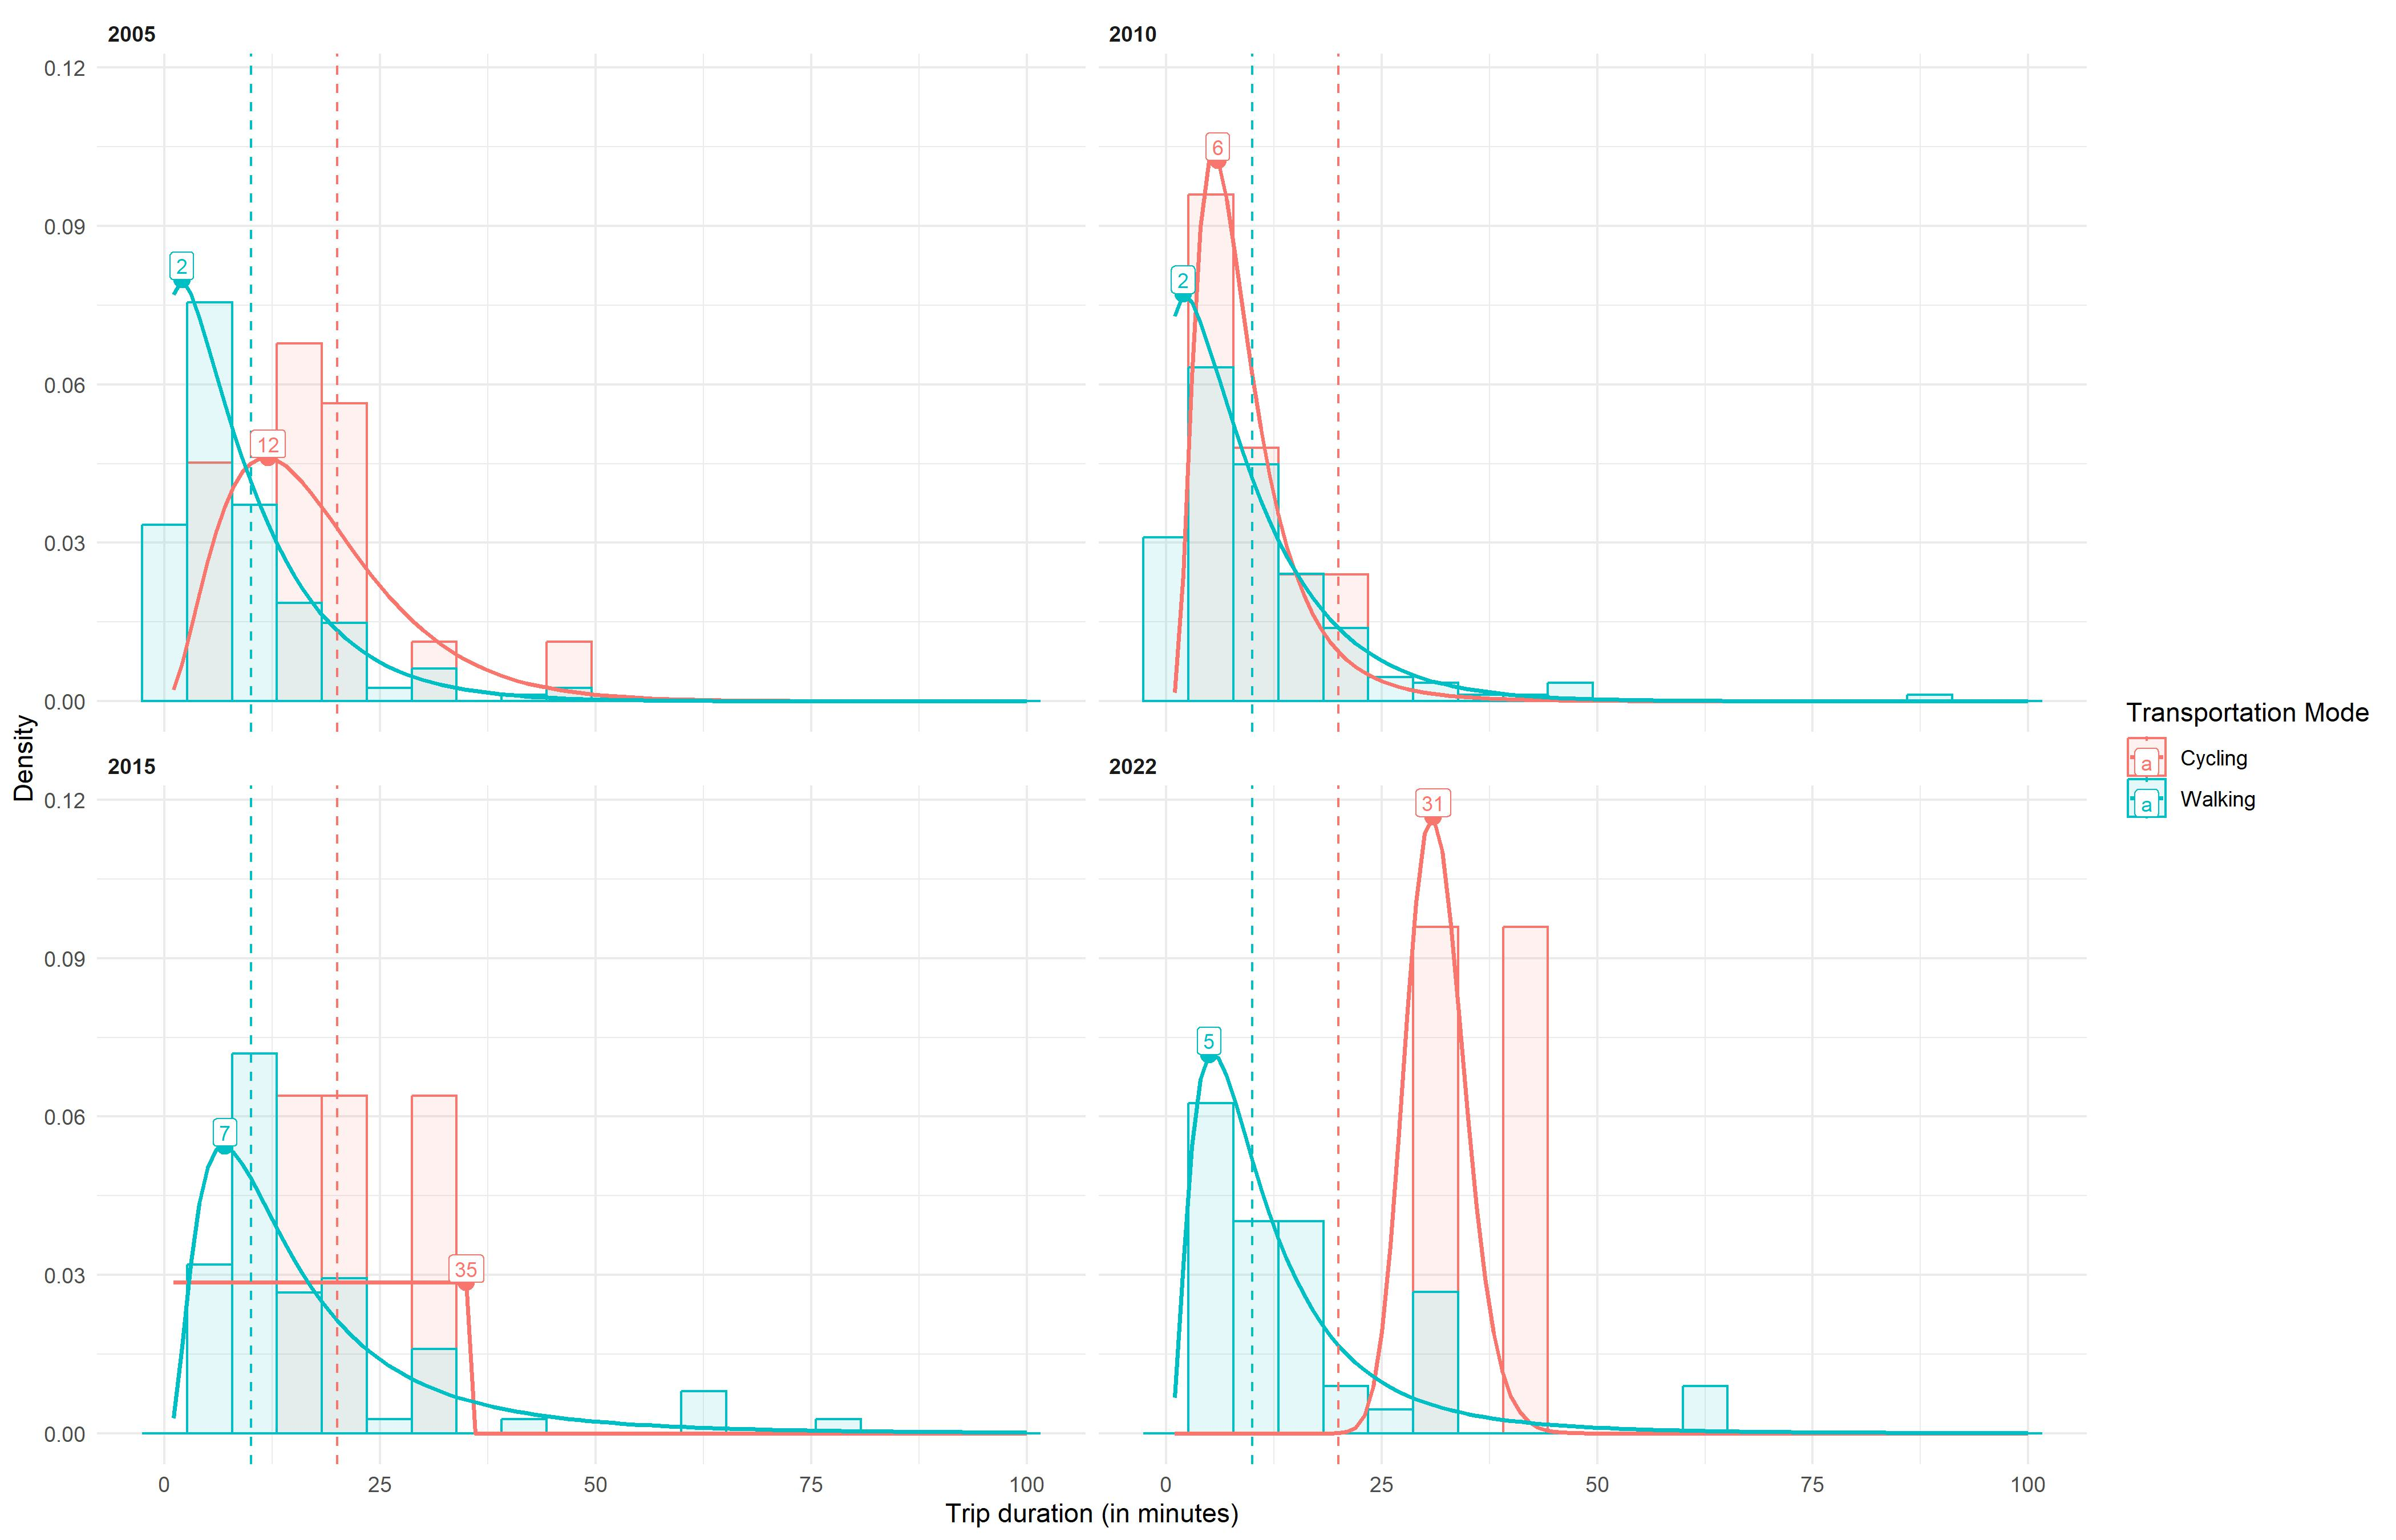
\includegraphics[width=1\linewidth]{figures/impf_Outdoors} 

}

\caption{Empirical data and impedance functions fitted for walking trips with `work or school` as destination.}\label{fig:outdoors-impedance-fig}
\end{figure}

For the years 2005 and 2010, the selected impedance functions are of the
gamma type, with shapes of \(\alpha = 1.24\) and \(\alpha = 1.27\),
respectively, and the same rate of \(\sigma = 0.13\). The rate parameter
(\(\sigma\)) mainly controls the speed of the curved drop, which is the
same for both years. The shape parameter (\(\mu\)) controls how the
density peak shifts in relation to the \(x\)-axis (the travel time). A
larger shape value means that the probability peak occurs at larger
values of time. Since the shape values for 2005 and 2010 are very close,
the peak of the PDF curve in both cases occurs at 2 minutes. Although
the difference in shape (\(\mu\)) between the two years is small and
does not change the time at which the peak occurs, it is enough to cause
a difference in the peak values themselves. In 2005, the walking trips
had a higher density around 2 minutes (0.079) compared to 2010 (0.077).

For 2015 and 2022, the PDFs that best represent the population's
transport behavior are lognormal distributions, with a mean of
\(\mu = 2.54\) and a standard deviation of \(\sigma = 0.79\) for 2015,
and a mean of \(\mu = 2.27\) and a standard deviation of
\(\sigma = 0.77\) for 2022. In 2015, the density peak (0.05) occurs at a
journey duration of 7 minutes. Here, we observe that a lower density
peak corresponds to a more dispersed curve, with higher densities at
longer durations. In fact, while in 2005 and 2010 walking trips had
densities close to zero for durations over 50 minutes, in 2015 there is
still a small density (0.002) at the 50-minute mark. In 2022, the
density peak (0.07) occurs at a duration of 5 minutes, and the curve is
less dispersed than in 2015, registering lower densities near the
50-minute mark (0.01), in comparison.

For trips made by bicycle, the best-fitting impedance function in 2005
is of the gamma type. For 2010 and 2022, the impedance functions are
best represented by lognormal distributions. In 2015, the PDF that best
fits the data is a uniform distribution, with an upper bound of 35
minutes and a peak density of 0.028. The presence of uniform functions
means that it was not possible to parameterize more complex functions
(like the other functions) and is explained by the low number of
episodes in this category of destination, mode of transport and year (in
this case, there were only 3 episodes identified). Overall, all the
uniform functions have a maximum of 6 episodes and all of them are for
the transportation mode cycling - which can be explained since this mode
of transport does not have many episodes compared to the walking
episodes (only 7\% of active travel episodes). The figure also shows how
cycling trips tend to have greater dispersion and higher typical values
(dashed vertical lines) when compared to walking trips.

The complexity of the impedance function depends on the number of
episodes available for calibration. For instance, fitting a gamma-type
function required an average of 219 episodes, while fitting a lognormal
function required approximately 176 episodes. In contrast, fitting a
normal function required only 5 episodes, and fitting a uniform function
required, on average, just 4 episodes.

The temporal difference between the decay functions is also evident in
Figure \ref{fig:walking-evolution-fig}, which shows the calibrated
functions for each year of analysis across all destination and transport
mode categories for walking trips. For some locations, the impedance
functions are of the same type and have similar parameters across all
the years analyzed. For example, the ``Cultural venues'', consistently
uses a gamma function to represent the population's transport behavior
for all the years analyzed. In this case, we observe that the average
cost is increasing, as the peaks of the PDFs are occurring at longer
durations and the curves are shifting to the right. This temporal trend
is primarily captured by the \(\sigma\) parameter (rate), which
decreased from 4.10 in 2005 to 3.89 in 2022. In contrast, the ``Place of
worship'' destination shows distinct temporal variations, with
noticeable changes in peak positions and density dispersion, reflecting
the empirical differences observed in Figure \ref{fig:figure-boxplot}
and discussed above. The most notable change in this second case is the
emergence of a uniform distribution, suggesting that the total number of
trips to this destination has declined over time.

\begin{figure}

{\centering 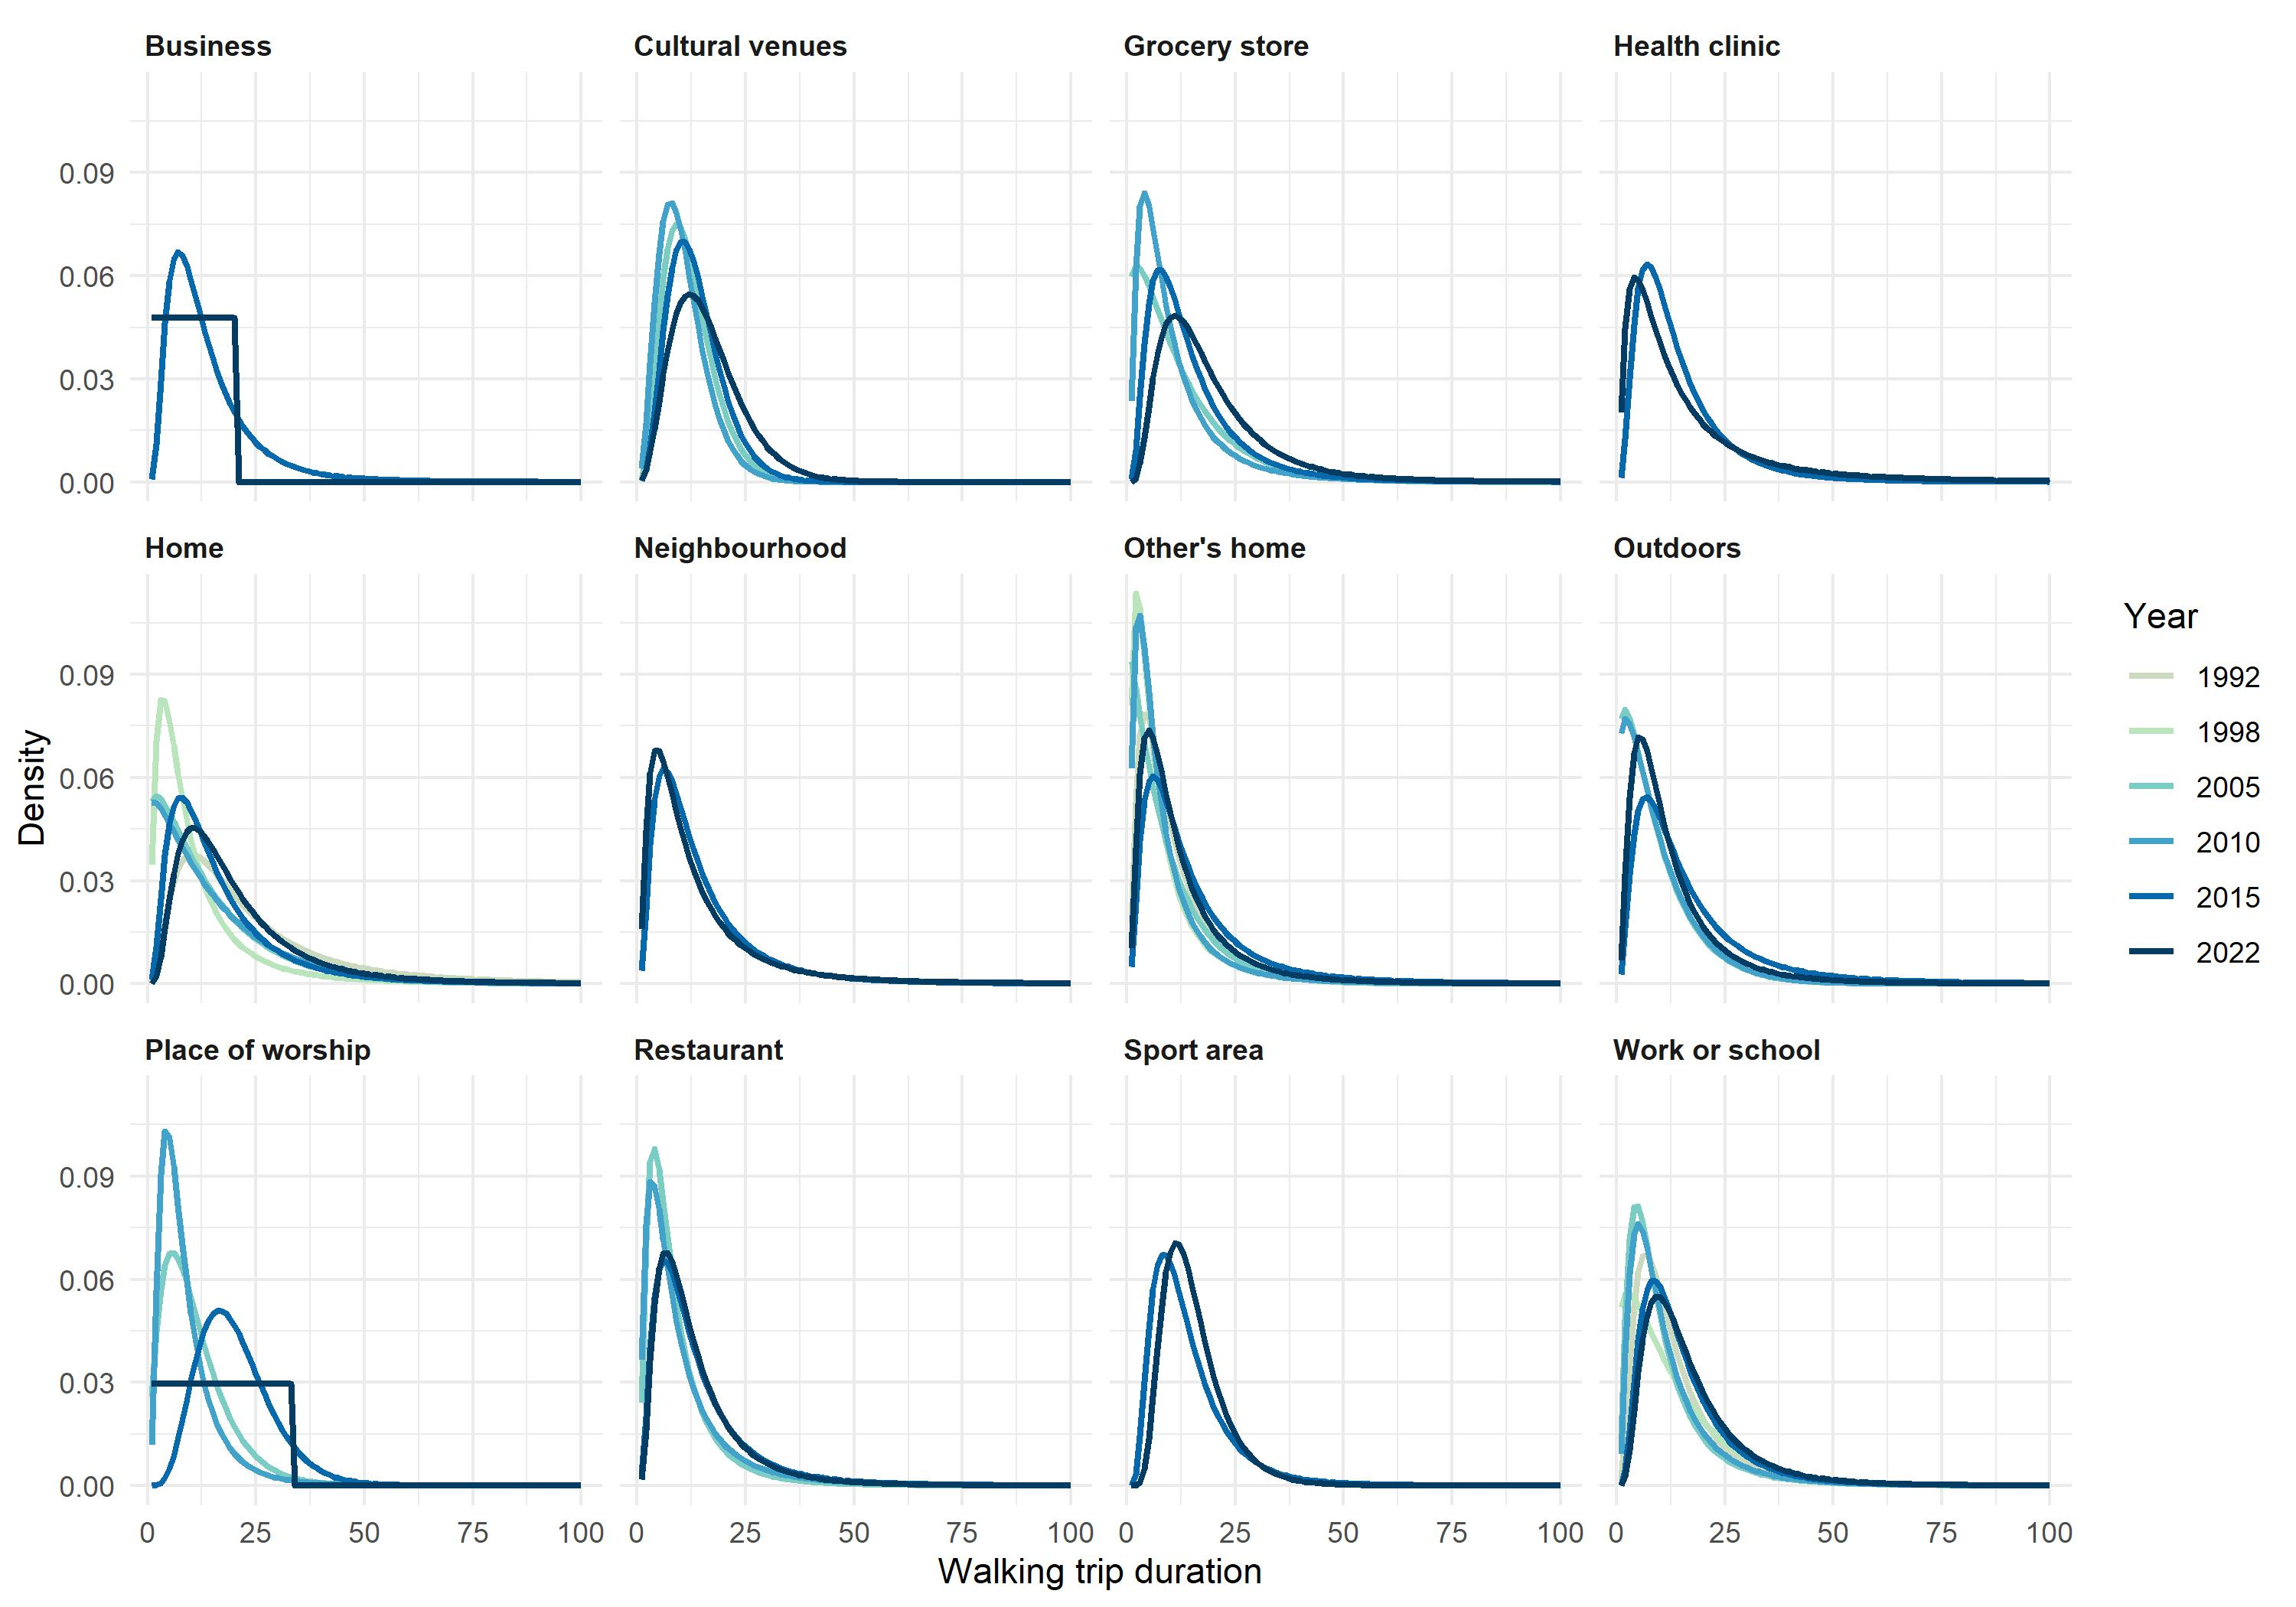
\includegraphics[width=1\linewidth]{figures/walking_temporal_evolution} 

}

\caption{Temporal evolution of walking impedance functions.}\label{fig:walking-evolution-fig}
\end{figure}

\section{Summary and conclusion}\label{summary-and-conclusion}

The main objectives of this study were to provide an overview of AT in
Canadian metropolitan cities, focusing on main origins, destinations,
travel times and active population on terms of age group and sex, and to
identify appropriate impedance functions for AT modes across various
destinations and time periods. In this study we perform a direct
application of \texttt{ActiveCA} R package \citep{dossantos2025},
analyzing over 13,500 cases of active travel trips that represented
28,066,620 episodes, from the Time Use cycles of the General Social
Survey (GSS) from 1992 to 2022, covering a twelve different type of
destinations and considering walking and cycling as transportation
modes.

The rate of active trips per person with active record was around two
trips, with an increasing trend in active episodes per person being
observed for both walking and cycling. Historically, men+ recorded more
active episodes than Women+, but in 2022 this trend reversed: men+
averaged 2.07 episodes, while women+ averaged 2.11. This change was
driven by a decrease in walking episodes among men+ (from 2.16 in 2015
to 2.07 in 2022) and an increase among women+ (from 1.92 to 2.11 in the
same period).

Our results show that the typical duration of walking trips increased to
15 minutes by 2022, following years of stability at 10 minutes. For
cycling, the typical duration rose to 30 minutes, recovering from a
decline that began in 1998 and lasted until 2010. Generally, walking
trips had consistently shorter durations than cycling trips. Although
this study does not explain the causes of these fluctuations, the
differences by year and mode were statistically significant.

When analyzed by gender, men+ increased their median cycling trip
duration from 15 minutes in 2005 to 30 minutes in 2022. Women+ increased
their median from 10 to 15 minutes. No gender differences were
identified in the duration of walking trips. When analyzing by age
groups, all of them increased their active travel times compared to
1992, especially for walking. For cycling, a marked increase in duration
emerged after 2010.

For both transportation modes trips to ``Other's home'' declined over
time, likely reflecting changing social behavior enabled by technology
that allows people to stay connected without visiting in person. Walking
trips were predominantly associated with ``Home'' as either the origin
or destination. For cycling, the combination of ``Home'' and ``Work or
school'' accounted for the majority of trips. Walking trip durations to
``Restaurants'' and ``Outdoors'' increased from 5 minutes in 2005 to 10
minutes in 2022. Travel to ``Places of worship'' also rose from 10
minutes in 2005 to 20 minutes in 2022, tying with ``Cultural venues''
for the highest typical walking travel time. Walking times to ``Home''
and ``Work or school'' increased to 15 minutes in 2022, following three
GSS cycles where they remained stable at 10 minutes. For cycling, 2015
marked the beginning of a trend toward longer travel times across nearly
all destinations.

The share of the population with at least one recorded active trip
ranged from a low of 6.93\% in 1998 to a peak of 15.06\% in 2010. In the
most recent GSS survey (2022), participation dropped to 9.45\%. Walking
dominated active trips, representing over 90\% of all episodes.

Since 2010, the active population has declined for both genders, with a
steeper decrease among women+. This reversed a long-standing pattern in
which women+ had higher AT participation than Men+. In 2022, men+ showed
higher prevalence than women+ regardless of mode, with 10.05\% for men+
and 8.84\% for Women+. In summary, women+ made more active trips, while
men+ had higher overall participation in AT.

Regarding age cohorts, the youngest group (15 to 24 years) remained the
most active, with a prevalence of 21.47\% in 2022. This was the only
group to show increased participation over the past decade, up from
17.91\% in 2015. Generally, AT prevalence decreases with age. However,
in both 2005 and 2022, the oldest group (75 years and older) reported
the third-highest AT prevalence (7.02\%) and showed a steady increase in
active episodes since 2010.

The study underscores the importance of applying destination-specific
impedance functions when measuring cost decay effects in accessibility
analyses. To this end, we fitted 83 impedance functions for AT trips
over a 30-year period, considering destination types and transportation
modes. The results indicate that none of the fitted functions followed
an exponential distribution, suggesting that commonly used functions in
AT accessibility studies may not adequately capture actual behavior -
especially for very short trips (under 5 minutes), which tend to be
overrepresented in these models. Destinations with many episodes were
best modeled using gamma functions, followed by lognormal and normal
distributions. In contrast, destinations with fewer than six episodes
were best represented by uniform distributions.

Given similarities in urbanization processes between Canada, the United
States, Australia, and West Europe, these findings may also be
applicable to metropolitan areas in those regions. Finally, this study
contributes to the ongoing discussion on AT, emphasizing its importance
in promoting sustainable transportation planning.

\section*{CRediT authorship contribution
statement}\label{credit-authorship-contribution-statement}
\addcontentsline{toc}{section}{CRediT authorship contribution statement}

\emph{(include after the review)}

\section*{Funding sources}\label{funding-sources}
\addcontentsline{toc}{section}{Funding sources}

This research was funded through project \emph{project name provided
after review)}, supported by the Social Sciences and Humanities Research
Council of Canada.

\section*{Data availability}\label{data-availability}
\addcontentsline{toc}{section}{Data availability}

We updated the \texttt{ActiveCA} R Package to include the methodology to
obtain impedance functions from the raw data files (GSS surveys).
Additionally, we created this paper using literate programming in which
the R markdown code to fully reproduce this article is available on our
GitHub repository \emph{(include after the review)}.

\section{Declaration of competing
interest}\label{declaration-of-competing-interest}

The authors declare no conflicts of interest

\section*{Appendix}\label{appendix}
\addcontentsline{toc}{section}{Appendix}

\renewcommand{\thetable}{A.1}

\begingroup\fontsize{8}{10}\selectfont

\begin{longtable}[t]{llllllll}
\caption{\label{tab:kruskal-walking}\label{tab:result-stats}P-values of the pairwise Wilcoxon test.}\\
\toprule
Mode & Destination & Year & 1992 & 1998 & 2005 & 2010 & 2015\\
\midrule
 & Home & 1998 & 0.00e+00 &  &  &  & \\
\nopagebreak
 & Home & 2005 & 0.00e+00 & 0.00e+00 &  &  & \\
\nopagebreak
 & Home & 2010 & 0.00e+00 & 0.00e+00 & 0.00e+00 &  & \\
\nopagebreak
 & Home & 2015 & 0.00e+00 & 0.00e+00 & 0.00e+00 & 0.00e+00 & \\
\nopagebreak
 & Home & 2022 & 0.00e+00 & 0.00e+00 & 0.00e+00 & 0.00e+00 & 0.00e+00\\
\nopagebreak
 & Work or school & 1998 & 7.09e-211 &  &  &  & \\
\nopagebreak
 & Work or school & 2005 & 0.00e+00 & 0.00e+00 &  &  & \\
\nopagebreak
 & Work or school & 2010 & 0.00e+00 & 0.00e+00 & 0.00e+00 &  & \\
\nopagebreak
 & Work or school & 2015 & 0.00e+00 & 0.00e+00 & 0.00e+00 & 0.00e+00 & \\
\nopagebreak
 & Work or school & 2022 & 0.00e+00 & 0.00e+00 & 0.00e+00 & 0.00e+00 & 0.00e+00\\
\nopagebreak
 & Grocery store & 2010 &  &  & 0.00e+00 &  & \\
\nopagebreak
 & Grocery store & 2015 &  &  & 0.00e+00 & 0.00e+00 & \\
\nopagebreak
 & Grocery store & 2022 &  &  & 0.00e+00 & 0.00e+00 & 0.00e+00\\
\nopagebreak
 & Neighbourhood & 2022 &  &  &  &  & 0.00e+00\\
\nopagebreak
 & Sport area & 2022 &  &  &  &  & 0.00e+00\\
\nopagebreak
 & Outdoors & 2010 &  &  & 4.33e-29 &  & \\
\nopagebreak
 & Outdoors & 2015 &  &  & 0.00e+00 & 0.00e+00 & \\
\nopagebreak
 & Outdoors & 2022 &  &  & 0.00e+00 & 0.00e+00 & 0.00e+00\\
\nopagebreak
 & Restaurant & 2010 &  &  & 2.09e-295 &  & \\
\nopagebreak
 & Restaurant & 2015 &  &  & 0.00e+00 & 0.00e+00 & \\
\nopagebreak
 & Restaurant & 2022 &  &  & 0.00e+00 & 0.00e+00 & 1.11e-179\\
\nopagebreak
 & Other's home & 1998 & 0.00e+00 &  &  &  & \\
\nopagebreak
 & Other's home & 2005 & 0.00e+00 & 1.79e-83 &  &  & \\
\nopagebreak
 & Other's home & 2010 & 0.00e+00 & 0.00e+00 & 0.00e+00 &  & \\
\nopagebreak
 & Other's home & 2015 & 0.00e+00 & 0.00e+00 & 0.00e+00 & 0.00e+00 & \\
\nopagebreak
 & Other's home & 2022 & 0.00e+00 & 0.00e+00 & 0.00e+00 & 0.00e+00 & 0.00e+00\\
\nopagebreak
 & Health clinic & 2022 &  &  &  &  & 4.12e-216\\
\nopagebreak
 & Cultural venues & 2010 &  &  & 4.52e-273 &  & \\
\nopagebreak
 & Cultural venues & 2015 &  &  & 0.00e+00 & 0.00e+00 & \\
\nopagebreak
 & Cultural venues & 2022 &  &  & 0.00e+00 & 0.00e+00 & 0.00e+00\\
\nopagebreak
 & Place of worship & 2010 &  &  & 0.00e+00 &  & \\
\nopagebreak
 & Place of worship & 2015 &  &  & 0.00e+00 & 0.00e+00 & \\
\nopagebreak
 & Place of worship & 2022 &  &  & 0.00e+00 & 0.00e+00 & 3.76e-18\\
\nopagebreak
\multirow[t]{-34}{*}{\raggedright\arraybackslash Walking} & Business & 2022 &  &  &  &  & 1.18e-305\\
\cmidrule{1-8}\pagebreak[0]
 & Grocery store & 2010 &  &  & 0.00e+00 &  & \\
\nopagebreak
 & Grocery store & 2015 &  &  & 0.00e+00 & 0.00e+00 & \\
\nopagebreak
 & Grocery store & 2022 &  &  & 0.00e+00 & 0.00e+00 & 0.00e+00\\
\nopagebreak
 & Home & 1998 & 1.08e-230 &  &  &  & \\
\nopagebreak
 & Home & 2005 & 1.45e-24 & 0.00e+00 &  &  & \\
\nopagebreak
 & Home & 2010 & 0.00e+00 & 0.00e+00 & 0.00e+00 &  & \\
\nopagebreak
 & Home & 2015 & 0.00e+00 & 8.44e-236 & 0.00e+00 & 0.00e+00 & \\
\nopagebreak
 & Home & 2022 & 0.00e+00 & 0.00e+00 & 0.00e+00 & 0.00e+00 & 0.00e+00\\
\nopagebreak
 & Work or school & 1998 & 0.00e+00 &  &  &  & \\
\nopagebreak
 & Work or school & 2005 & 9.62e-228 & 0.00e+00 &  &  & \\
\nopagebreak
 & Work or school & 2010 & 1.30e-221 & 0.00e+00 & 0.00e+00 &  & \\
\nopagebreak
 & Work or school & 2015 & 0.00e+00 & 0.00e+00 & 0.00e+00 & 0.00e+00 & \\
\nopagebreak
 & Work or school & 2022 & 0.00e+00 & 0.00e+00 & 0.00e+00 & 0.00e+00 & 0.00e+00\\
\nopagebreak
 & Health clinic & 2022 &  &  &  &  & 0.00e+00\\
\nopagebreak
 & Restaurant & 2010 &  &  & 1.03e-106 &  & \\
\nopagebreak
 & Restaurant & 2015 &  &  & 0.00e+00 & 0.00e+00 & \\
\nopagebreak
 & Restaurant & 2022 &  &  & 0.00e+00 & 0.00e+00 & 0.00e+00\\
\nopagebreak
 & Sport area & 2022 &  &  &  &  & 0.00e+00\\
\nopagebreak
 & Outdoors & 2010 &  &  & 0.00e+00 &  & \\
\nopagebreak
 & Outdoors & 2015 &  &  & 0.00e+00 & 0.00e+00 & \\
\nopagebreak
 & Outdoors & 2022 &  &  & 0.00e+00 & 0.00e+00 & 0.00e+00\\
\nopagebreak
 & Other's home & 1998 & 2.60e-122 &  &  &  & \\
\nopagebreak
 & Other's home & 2005 & 0.00e+00 & 0.00e+00 &  &  & \\
\nopagebreak
 & Other's home & 2010 & 6.63e-41 & 0.00e+00 & 3.60e-287 &  & \\
\nopagebreak
 & Other's home & 2015 & 4.03e-81 & 0.00e+00 & 5.62e-266 & 1.84e-148 & \\
\nopagebreak
 & Cultural venues & 2010 &  &  & 2.98e-142 &  & \\
\nopagebreak
\multirow[t]{-27}{*}{\raggedright\arraybackslash Cycling} & Cultural venues & 2015 &  &  & 0.00e+00 & 9.65e-01 & \\
\bottomrule
\end{longtable}
\endgroup{}

\renewcommand\refname{References}
\bibliography{mybibfile2}


\end{document}
